\documentclass[12pt, a4paper, twoside, openright]{report}

% Idioma y títulos
\usepackage[spanish, es-nodecimaldot, es-noquoting]{babel}
\addto\captionsspanish{\renewcommand{\bibname}{Referencias consultadas}}

\usepackage{tikz,tikz-3dplot,tkz-euclide}
\usetikzlibrary{positioning, arrows.meta, shadows, shapes.geometric, shapes.symbols, calc}

% Codificación y fuentes
\usepackage[utf8]{inputenc}
\usepackage[T1]{fontenc}
\usepackage{palatino}

% Matemáticas y teoremas
\usepackage{amsmath, amsthm, amsfonts, mathtools}

% Gráficos y dibujo
\usepackage{graphicx}

% Tablas/variado
\usepackage{booktabs}
\usepackage{enumerate}
\usepackage{float}
\usepackage{microtype}
\usepackage{listings}
\usepackage[margin=2.5cm]{geometry}
\usepackage{setspace}
\onehalfspacing

% Páginas en blanco al cerrar un capítulo (recto/verso)
% emptypage hace que las páginas auto-insertadas al final de un capítulo
% queden totalmente en blanco (sin encabezado ni número), de modo que el
% siguiente capítulo siempre comience en página derecha.
\usepackage{emptypage}

% Colores y enlaces
\usepackage{xcolor}
\definecolor{mypurple}{HTML}{622567}
\definecolor{myred}{HTML}{D55C19}
\definecolor{myblue}{HTML}{007A87}
\usepackage[colorlinks,linkcolor=myblue,citecolor=mypurple]{hyperref}

% Encabezados y formato de capítulos
\usepackage{fancyhdr,titlesec}
\renewcommand{\baselinestretch}{1.5}

% Entornos de teoremas
\theoremstyle{plain}
\newtheorem{theorem}{Theorem}[chapter]
\newtheorem{lemma}[theorem]{Lemma}
\newtheorem{proposition}[theorem]{Proposition}
\newtheorem{corollary}[theorem]{Corollary}
\theoremstyle{definition}
\newtheorem{definition}[theorem]{Definition}
\newtheorem{example}[theorem]{Example}
\newtheorem{remark}{Nota}
\newtheorem{assumption}{Supuesto}

% ==========================================
% DEFINICIONES DE VARIABLES (Poner en el Preámbulo)
% ==========================================
\newcommand{\IHED}{I_{\text{HED}}} % Componente Hedónico
\newcommand{\IACC}{I_{\text{ACC}}} % Accesibilidad
\newcommand{\ISEG}{I_{\text{SEG}}} % Seguridad
\newcommand{\IDOT}{I_{\text{DOT}}} % Dotacional
\newcommand{\IPNU}{I_{\text{PNU}}} % Potencial Normativo
\newcommand{\IUG}{IUG}             % Índice Global

\usepackage[round]{natbib} % 'round' pone paréntesis redondos ()
% Encabezados
\pagestyle{fancy}
\setlength{\headheight}{15.5pt}
\fancyheadoffset[LE,RO]{0pt}
\renewcommand{\chaptermark}[1]{\markboth{#1}{}}
\renewcommand{\sectionmark}[1]{\markright{\thesection\ #1}}
\fancyhf{}
\fancyhead[LE]{\makebox[0pt][l]{\thepage}\hfill\leftmark}
\fancyhead[RO]{\rightmark\hfill\makebox[0pt][r]{\thepage}}
\fancypagestyle{plain}{\fancyhead{}\renewcommand{\headrulewidth}{0pt}}

% Formato de capítulos
\titleformat{\chapter}[display]
    {\normalfont\bfseries\color{myred}}
    {\filleft\hspace*{-60pt}%
        \rotatebox[origin=c]{90}{%
            \normalfont\color{black}\Large%
            \textls[180]{\textsc{\chaptertitlename}}%
        }\hspace{10pt}%
        {\setlength\fboxsep{0pt}%
            \colorbox{myred}{\parbox[c][3cm][c]{2.5cm}{%
                \centering\color{white}\fontsize{80}{90}\selectfont\thechapter}}
        }}
    {10pt}
    {\titlerule[2.5pt]\vskip3pt\titlerule\vskip4pt\LARGE\sffamily}

\begin{document}

%%%%%%%%%%%% BEGIN TITLE PAGE %%%%%%%%%%%%

\thispagestyle{empty} % For the title page, no header / footer

\noindent
    \begin{minipage}{0.1\textwidth}
    \includegraphics[height=4 cm]{logoPUJ.png}
    \end{minipage}
    \hfill
    \begin{minipage}{0.5\textwidth}
    \begin{center}
        \renewcommand\familydefault{\sfdefault}
        \fontfamily{phv}\selectfont
        {\large Facultad de Ciencias\\Departamento de Matem\'aticas}
    \end{center}
    \end{minipage}

\begin{center}
    \noindent\textcolor{myred}{\rule{\linewidth}{4.8pt}}
    
    \vspace{2em}
    \noindent {\LARGE \sc Programa Ciencia de Datos\\Trabajo de Grado}
    
    \vspace{3em}
    \noindent {\Huge{\color{myblue} \'Indice de Precios Inmobiliarios por
Bienestar y Entorno Urbano}}
    
    \vspace{3em}
    \noindent {\Large \bf NEYL PEÑUELA BERNATE}
    \vfill
    \noindent {\Large {Director:} {\color{mypurple} \bf Vladimir Moreno G.}}
    
    \vspace{0.5em}
    \noindent\textcolor{myred}{\rule{\linewidth}{4.8pt}}
    
    \vspace{2em}
    {\Large \today }
    
    {\Large Bogot\'a, Colombia}
\end{center}
\newpage

\vspace{10cm}

\begin{center}

 \includegraphics[scale=3.0]{selloagua.pdf}  
    \end{center}



\clearpage

%%%%%%%%%%%% END TITLE PAGE %%%%%%%%%%%%

%%%%%%%%%%%% BEGIN DEDICATORIA %%%%%%%%%%%%
\thispagestyle{empty}
\cleardoublepage
\thispagestyle{empty}

\vspace*{\fill}
\begin{flushright}
    \begin{minipage}{0.65\textwidth}
        \begin{flushright}
            {\fontfamily{pzc}\selectfont\Huge\color{mypurple} Dedicatoria}\\[2.5em]
            {\Large\itshape
            % --- Escribe aquí tu dedicatoria ---
            \phantom{Texto de dedicatoria. Reemplaza este párrafo}\\[0.8em]
            \phantom{por las palabras que quieras dedicar a las}\\[0.8em]
            \phantom{personas que te acompañaron en este camino.}
            % --- Fin del bloque editable ---
            }
        \end{flushright}
    \end{minipage}
\end{flushright}
\vspace*{\fill}

\cleardoublepage
%%%%%%%%%%%% END DEDICATORIA %%%%%%%%%%%%

\tableofcontents

% If you have lots of figures with captions / numbers, uncomment the following line
% \listoffigures

% If you have lots of tables and want a list of them, uncomment the following line
% \listoftables
% --- Macros útiles ---
\newcommand{\ratio}{\textit{ratio}}% palabra "ratio" siempre en cursiva

% ==========================================
% CAPÍTULO 1: INTRODUCCIÓN
% ==========================================
\chapter{Introducción}\label{ch:intro}
\section{Contexto y Motivación}

El mercado de finca raíz ha constituido tradicionalmente un vehículo fundamental de ahorro e inversión en Colombia, y específicamente Bogotá se ha visto inundada por este manejo de los inmuebles. Históricamente, agentes económicos de diversa escala, desde pequeños propietarios hasta grandes fondos de inversión, han diversificado sus portafolios mediante activos inmobiliarios, bajo la premisa de que estos ofrecen estabilidad temporal, baja volatilidad y resiliencia frente a las fluctuaciones macroeconómicas.


No obstante, la valoración residencial se plantea como un desafío técnico y económico. Pues en si, la vivienda es un activo inherentemente heterogéneo y con alta especificidad espacial; su valor de mercado no solo responde a las características físicas de la estructura, sino que es función de las preferencias de los avaluadores, las condiciones del entorno inmediato y una serie de atributos urbanos (seguridad, accesibilidad, normativa) que frecuentemente resultan subrepresentados en las metodologías de valoración convencionales y hasta subjetivos. En la literatura especializada, tomando por ejemplo el enfoque hedónico que conceptualiza el valor del bien como la suma de los precios implícitos de sus características, se ha establecido como el vehículo central para explicar la formación de precios \citep{rosen1974}.


Finalmente, reconociendo que la interpretación de estos datos urbanos puede ser compleja por su alta dimensionalidad el proyecto contempla una fase de despliegue tecnológico mediante metodologías de Inteligencia Artificial Generativa. En la que se aprovecha la capacidad de modelos de lenguaje avanzados y la riqueza de los datos no estructurados de los inmuebles para habilitar un asistente conversacional, permitiendo consultar un indicador que represente información objetiva y encontrar oportunidades de inversión mediante lenguaje natural.


\section{Planteamiento del IUG}

En este contexto, el presente trabajo propone el desarrollo del Índice Urbano Global (\IUG{}) como una herramienta de análisis estadístico poblacional para Bogotá. La base empírica del estudio compila un extenso dataset de anuncios de vivienda publicados en portales de alta penetración en el mercado. Si bien esta muestra no alcanza el universo transaccional total, captura una porción estadísticamente significativa de la oferta efectiva, permitiendo una trazabilidad espacial detallada a nivel de Barrio y Localidad.



El \IUG{} contribuye no solo a explicar la varianza en los precios, sino a medir la calidad integral del activo inmobiliario de manera independiente al valor monetario. El índice sintetiza cinco dimensiones críticas:

\begin{itemize}

    \item \textbf{Componente Hedónico (Calidad Intrínseca):} Evalúa las especificaciones propias del inmueble, considerando tanto su dimensión espacial (área construida, distribución) como sus atributos físicos y de confort.

    \item \textbf{Seguridad objetiva y entorno:} Medición basada en datos históricos de incidencia delictiva (GeoJSON) y percepción ciudadana.

    \item \textbf{Accesibilidad y movilidad:} Oferta de transporte público (SITP/TransMilenio) y conectividad vial.

    \item \textbf{Proximidad a puntos de interés (Dotacionales):} Cercanía a servicios de salud, educación, abastecimiento y espacio público.

    \item \textbf{Potencial normativo:} Capacidad de edificabilidad y lineamientos de planeación urbana (POT).

\end{itemize}


\section{Objetivos de la Investigación}
\label{sec:objetivos}

\subsection{Objetivo General}

Diseñar, implementar y validar el \textbf{\IUG} como una herramienta poblacional, abierta y reproducible que sintetice cinco dimensiones del bienestar urbano de Bogotá en una métrica única. Este indicador operará como un sistema de soporte a la decisión inmobiliaria, calculado de forma estrictamente independiente al precio de mercado.

\subsection{Objetivos Específicos}

\begin{enumerate}
    \item \textbf{Operacionalizar} las dimensiones de accesibilidad, seguridad, calidad construida, dotación y potencial normativo en subíndices comparables, utilizando fuentes oficiales abiertas (DANE, IDECA, SDP, POT 555, EPV 2024, ICSU).
    
    \item \textbf{Construir un pipeline de datos reproducible} que integre la extracción automatizada de oferta inmobiliaria, asignaciones espaciales a nivel de bases de datos, control de calidad mediante algoritmos de agrupación y persistencia versionada, garantizando la trazabilidad desde el anuncio hasta el indicador final.
    
    \item \textbf{Estimar un modelo hedónico de referencia} (OLS, Ridge, Lasso, Elastic Net) cuyo propósito exclusivo es servir como \emph{base line} descriptivo para contrastar la información incremental que aporta el \IUG{}.
    
    \item \textbf{Validar estadísticamente el indicador} mediante un protocolo de once pruebas que evalúe su bondad de ajuste, robustez, validez convergente y de uso.
    
    \item \textbf{Cuantificar la incertidumbre} del índice mediante descomposición de varianza (índices de Sobol) y análisis de sensibilidad ante perturbación Monte Carlo de sus pesos.
    
    \item \textbf{Habilitar el acceso operativo} mediante un despliegue web público y un asistente conversacional (RAG) que democratice la consulta del indicador sin requerir conocimientos técnicos en geoestadística.
\end{enumerate}

\section{Pregunta de Investigación y Postura Metodológica}

Para materializar estos objetivos, es fundamental resolver la siguiente cuestión central: \textit{¿Es posible construir, a partir de fuentes abiertas y replicables, un indicador sintético de calidad urbana que sea estadísticamente válido, robusto y operativamente útil para identificar discrepancias entre el precio observado y los fundamentales urbanos del territorio?}

Para responderla, esta tesis asume una postura metodológica deliberadamente \emph{descriptiva-decisional}, y no predictiva. Un señalamiento natural sobre cualquier métrica urbana es cuestionar qué tan bien predice el precio. Sin embargo, el \IUG{} \textbf{no se propone inferir, estimar ni predecir el precio de mercado} de un inmueble. Ya existen familias maduras de Modelos de Valoración Automática (AVM) que cumplen ese rol con métricas establecidas por la \textit{International Association of Assessing Officers} (IAAO, 2013). Estos estándares (COD, PRD y PRB) se desarrollan con detalle en la Sección~\ref{subsec:iaao_estandares} del Marco Teórico, y se retoman como diagnóstico del modelo hedónico de referencia en el Capítulo~\ref{ch:resultados}. 

La propuesta del \IUG{} es funcionar como una \textbf{herramienta-perspectiva}: un instrumento analítico que condensa cinco metodologías heterogéneas en una escala interpretable y ortogonal al precio. Su virtud no reside en la correlación con el valor comercial, sino en su capacidad de revelar la brecha existente entre lo que el mercado paga y la calidad objetiva del entorno.

\section{Hipótesis y Alcance del Proyecto}

Este enfoque se sustenta en una \textbf{hipótesis central}: existe información estructural sobre la calidad urbana que el precio no captura íntegramente. A nivel operativo, se plantea que la ortogonalidad entre el \IUG{} y el precio (con una correlación débil esperada de $|\rho| < 0.30$) no es un defecto del modelo, sino la condición necesaria para que este aporte información nueva sobre el \emph{benchmark} hedónico.

Para delimitar con precisión el fin y alcance de este proyecto, es importante recalcar que esta tesis:

\begin{itemize}
    \item No sustituye la valoración profesional caso a caso ni estima precios puntuales para inmuebles individuales.
    \item No incorpora costos de obra, tasas de descuento ni evalúa estructuras financieras de proyectos (Método Residual Dinámico).
    \item No pretende fungir como instrumento tributario ni base catastral, ofreciendo un complemento analítico en lugar de una sustitución regulatoria.
    \item No pretende alcanzar eficiencia predictiva sobre el precio, ya que la divergencia con las métricas tradicionales es el núcleo que permite identificar discrepancias de valor.
\end{itemize}

\section{Contribución y Alcance Metodológico}

La idea central de la investigación es comparar el precio observado con un conjunto de fundamentales urbanos para reducir la subjetividad inherente a las valoraciones zonales. El alcance metodológico integra cuatro componentes: un \emph{benchmark} hedónico para establecer la línea base, la construcción del índice sintético multidimensional, un protocolo de validación estadística y un despliegue tecnológico final.

La relación entre las dimensiones de calidad y el mercado se materializa mediante el Ratio de Oportunidad, un instrumento diseñado para detectar \emph{mispricing} relativo:

\begin{equation}
    \text{Ratio} = \frac{\IUG{}}{\text{Precio Estandarizado}}
\end{equation}

Esta métrica ofrece valor directo a inversionistas y al sector financiero, permitiendo la identificación \emph{data-driven} de oportunidades (alto valor urbanístico y precios contenidos) o la emisión de alertas (baja calidad y precios elevados). Adicionalmente, subíndices específicos como el de seguridad ($I_{SEG}$) tienen aplicabilidad directa en el ámbito actuarial para modelos de frecuencia, severidad y tarificación geoespacial.

\paragraph{Reproducibilidad y código abierto.} El código fuente, la documentación técnica detallada, las instrucciones de despliegue local y las capturas representativas del sistema están disponibles públicamente en el repositorio del proyecto:

\begin{center}
\url{https://github.com/neylinsomne/indice-urbano-global-bogota}
\end{center}

\noindent La plataforma desplegada es accesible en \url{https://inmu.vara-alta.lat}. El detalle técnico completo se documenta en el Anexo~\ref{ax:tecnico}.
% ==========================================
% CAPÍTULO 2: MARCO TEÓRICO Y CONCEPTUAL
% ==========================================
\chapter{Marco Teórico}\label{ch:marco_teorico}

\section{Fundamentos Econométricos}

\subsection{Lo que ve el mercado: Regresión Lineal Múltiple}
El punto de partida para modelar el precio es la especificación lineal clásica. Sea $Y$ la variable respuesta (precio o log-precio) y $X_1,\dots,X_p$ los predictores (atributos). En notación matricial, el modelo se expresa como:
\begin{equation}
\mathbf{Y} = \mathbf{X}\boldsymbol{\beta} + \boldsymbol{\varepsilon}
\end{equation}
Donde:
\begin{itemize}
    \item $\mathbf{X} \in \mathbb{R}^{n\times (p+1)}$ es la matriz de diseño (incluyendo el intercepto).
    \item $\boldsymbol{\beta}=(\beta_0,\dots,\beta_p)^\top$ es el vector de coeficientes a estimar.
    \item $\boldsymbol{\varepsilon} \sim \mathcal{N}(\mathbf{0},\sigma^2\mathbf{I})$ es el término de error, bajo supuestos de independencia y homocedasticidad.
\end{itemize}

El estimador de Mínimos Cuadrados Ordinarios (MCO) está dado por $\hat{\boldsymbol{\beta}}=(\mathbf{X}^\top\mathbf{X})^{-1}\mathbf{X}^\top\mathbf{Y}$, siendo este el Mejor Estimador Lineal Insesgado (BLUE) bajo las condiciones de Gauss-Markov. En la práctica inmobiliaria, es crítico evaluar la linealidad, la normalidad de los residuos y, especialmente, la multicolinealidad entre atributos estructurales.

\subsection{Teoría de Precios Hedónicos}
La valoración residencial presenta complejidades derivadas de la heterogeneidad del activo. La Teoría de Precios Hedónicos, formalizada por \citet{rosen1974}, postula que los bienes heterogéneos son valorados por su conjunto de atributos de utilidad. El modelo descompone el precio total en la suma de los valores implícitos de sus características:
\begin{enumerate}
    \item \textbf{Estructurales:} Área, edad, acabados.
    \item \textbf{Vecindario:} Estrato, demografía.
    \item \textbf{Localización:} Accesibilidad, cercanía a CBD (Central Business District).
\end{enumerate}
Mientras que la estimación por MCO captura los efectos promedio, la \textbf{Regresión Cuantílica} permite revelar la heterogeneidad de estos efectos a lo largo de la distribución condicional del precio (ej. en los cuantiles $q_{10}, q_{50}, q_{90}$), reconociendo que el mercado de lujo puede valorar los atributos de forma distinta al mercado de vivienda de interés social.

\section{Enfoques de Valoración y Desarrollo Urbano}

\subsection{Valoración Masiva y Modelos Poblacionales}
En diversas jurisdicciones, la gestión tributaria y catastral ha migrado hacia esquemas de \emph{Valoración Masiva Automatizada} (AVM). Estos sistemas buscan consistencia y eficiencia mediante modelos econométricos calibrados con información transaccional y catastral. Este trabajo se alinea con este espíritu comparativo al estimar un modelo supervisado para caracterizar ``lo que ve el mercado'', pero innova al proponer el \IUG{} como una métrica independiente del precio para contrastar el valor observado con los fundamentales urbanos.

\subsection{Estándares IAAO para la calidad de los avalúos masivos}
\label{subsec:iaao_estandares}

La \textit{International Association of Assessing Officers} (IAAO) publica los estándares internacionales más extendidos para evaluar la calidad estadística de modelos de valoración masiva \citep{iaao2013}. Estos estándares se materializan en tres métricas que el Capítulo~\ref{ch:resultados} retoma al diagnosticar el modelo hedónico:

\begin{description}
    \item[\textbf{COD} (\textit{Coefficient of Dispersion}):] mide la \emph{uniformidad} de las estimaciones. Se calcula como el promedio de las desviaciones absolutas del cociente \mbox{(precio estimado / precio observado)} respecto a su mediana, expresado en porcentaje. Un COD bajo indica que el modelo trata de forma homogénea a inmuebles similares. La IAAO considera \textbf{aceptable un COD entre 5\,\% y 15\,\%} para vivienda residencial; valores superiores reflejan dispersión inherente al mercado que ningún modelo puede comprimir con datos de oferta.

    \item[\textbf{PRD} (\textit{Price-Related Differential}):] mide la \emph{equidad vertical} (\textit{progresividad / regresividad}). Se obtiene como el cociente entre la media aritmética y la media ponderada por valor de los ratios precio estimado/observado. Un \textbf{PRD en el rango $[0.98,\,1.03]$} indica neutralidad; valores $>1.03$ sugieren \emph{regresividad} (el modelo subvalora propiedades caras frente a baratas), mientras que valores $<0.98$ sugieren \emph{progresividad}.

    \item[\textbf{PRB} (\textit{Price-Related Bias}):] complementa al PRD con una medida más robusta de la misma equidad vertical, estimada como la pendiente de una regresión auxiliar entre el ratio precio/valor y el logaritmo del valor. La IAAO considera aceptables \textbf{valores en $[-0.05,\,+0.05]$}; pendientes mayores en magnitud confirman sesgo sistemático respecto al nivel de precio.
\end{description}

Estos tres estadísticos se complementan con el \emph{ratio mediano} (precio estimado / precio observado), que debe situarse en torno a 1.00 para garantizar la ausencia de sesgo global. En el presente trabajo se reportan los cuatro valores como diagnóstico del modelo hedónico (Cuadro~\ref{tab:iaao_res}) y no como criterio de aceptación del $\IUG{}$, dado que este último no se propone como AVM.

\subsection{El Método Residual Dinámico y su Relación con el IUG}
En el ámbito del desarrollo inmobiliario, la valoración de suelo o proyectos en curso suele realizarse mediante el \emph{Método Residual Dinámico}. Este enfoque calcula el valor actual del suelo partiendo del valor hipotético del proyecto terminado y descontando los costos de construcción, honorarios, financieros y la utilidad del promotor en el tiempo \citep{TasadorResidual}. Es especialmente útil para activos que aún no generan rentas o suelos urbanizables.

\begin{remark}[\textbf{Relación con este estudio}]
El enfoque residual es idóneo cuando el \emph{potencial edificatorio} es el driver principal del valor. En esta tesis, dicha dimensión se captura mediante el subíndice $I_{PNU}$ (Potencial Normativo–Urbanístico), que resume la capacidad edificatoria (índice de construcción) y los usos permitidos por el POT.
\\
Sin embargo, el \IUG{} no internaliza explícitamente costos de obra o tasas de descuento financiero; su función es complementaria. Mientras el método residual determina la viabilidad financiera de un proyecto específico, el \IUG{} y el ratio IUG/Precio ofrecen un \emph{baseline} espacial poblacional para detectar si el mercado está pagando por el suelo un precio acorde a su capacidad normativa y calidad urbana, independientemente de la estructura de costos de un desarrollador particular.
\end{remark}

\section{Dimensiones del Bienestar Urbano}

\subsection{Espacio Público y Seguridad}
El bienestar urbano trasciende la propiedad privada. El espacio público (zonas verdes, parques) y la seguridad (tanto objetiva, medida en tasas de criminalidad, como subjetiva/percibida) son determinantes en la disposición a pagar de los hogares. La literatura sugiere que la inseguridad actúa como un ``impuesto implícito'' sobre el valor de la vivienda, mientras que la accesibilidad peatonal y el transporte masivo generan plusvalías por localización.

\subsection{Econometría Espacial y Machine Learning}
Dado que "todo está relacionado con todo, pero las cosas cercanas están más relacionadas que las distantes" (Primera Ley de la Geografía, Tobler), los modelos inmobiliarios deben gestionar la dependencia espacial.
\begin{itemize}
    \item \textbf{Diagnóstico:} Uso del Índice de Moran para detectar autocorrelación en los residuos.
    \item \textbf{Exploración:} Técnicas de reducción de dimensionalidad como \textbf{PCA} (Análisis de Componentes Principales) para reducir la dimensionalidad de atributos correlacionados, y algoritmos de agrupamiento como \textbf{DBSCAN} para identificar ``clústeres'' espaciales de precios o anomalías que no siguen la lógica del mercado general.
\end{itemize}

% ==========================================
% SECCIÓN 2.4: MARCO CONCEPTUAL Y OPERATIVO
% ==========================================

\section{Marco Conceptual y Definiciones Operativas}
\label{sec:marco_conceptual}

A diferencia del marco teórico, que expone los fundamentos científicos generales, esta sección operacionaliza dichas teorías en variables específicas, estableciendo el sistema de ecuaciones del Índice Urbano Global (IUG) y los protocolos de manejo de datos.

\subsection{Definiciones Básicas del Estudio}
\begin{description}
    \item[\textbf{Inmueble (Unidad de Análisis):}] Anuncio georreferenciado de vivienda (Propiedad Horizontal o Casa) en Bogotá. El precio observado se estandariza como precio por metro cuadrado ($\tilde P_i$), ajustado por métricas de control.
    \item[\textbf{Barrio / Localidad:}] Unidades administrativas del Distrito Capital usadas como contenedores espaciales para la agregación de métricas zonales y validación geométrica.
    \item[\textbf{Modelo Hedónico:}] Especificación econométrica supervisada que explica el logaritmo del precio en función de los atributos. Representa \emph{lo que ve el mercado}.
    \item[\textbf{Índice Urbano Global (IUG):}] Indicador sintético adimensional (escala 0-5), \emph{independiente del precio}, que cuantifica la calidad integral del entorno urbano.
\end{description}

% -- FUSIÓN DE FÓRMULA, TABLA Y NORMALIZACIÓN --
\subsection{Construcción y Formulación Matemática del IUG}
\label{subsec:construccion_iug}

El modelo conceptual del índice se define como la combinación lineal ponderada de cinco dimensiones críticas del bienestar urbano. Para cada inmueble $i$, la formulación matemática se expresa como:

\begin{equation}
\IUG_i = w_1 I_{HED} + w_2 I_{ACC} + w_3 I_{SEG} + w_4 I_{DOT} + w_5 I_{PNU}
\end{equation}

Donde $\sum w_k = 1$. Cada uno de estos componentes ($I_k$) se calcula a partir de variables operativas específicas, detalladas en la Tabla \ref{tab:indicadores_conceptuales}.

\begin{table}[ht]
  \centering
  \caption{Definición operativa y dirección de los subíndices del IUG.}
  \label{tab:indicadores_conceptuales}
  \resizebox{\textwidth}{!}{%
  \begin{tabular}{@{}p{1.5cm} p{3.5cm} p{8.0cm} p{1.5cm}@{}}
    \toprule
    \textbf{Símbolo} & \textbf{Dimensión} & \textbf{Definición Operativa} & \textbf{Signo ($S$)}\\
    \midrule
    $I_{HED}$ & Calidad Intrínseca & \textbf{Score Hedónico:} Resultado de un PCA sobre variables estructurales (área, baños, garajes). Representa el confort privado. & + \\ \addlinespace
    
    $I_{ACC}$ & Accesibilidad & \textbf{Modelo Gravitacional:} Sumatoria de oportunidades ponderadas por el inverso de la distancia ($d_{ij}^{-\beta}$) a estaciones de TransMilenio y SITP. & + \\ \addlinespace
    
    $I_{SEG}$ & Seguridad & \textbf{Indicador Tridimensional:} Combina tres capas: (1)~de proximidad local (proximidad a CAI y sectores priorizados, peso 0.40), (2)~criminalidad objetiva ICSU con 7 tipos de delito normalizados por km$^2$ (peso 0.30), y (3)~percepción subjetiva derivada de la EPV 2024 (peso 0.30). & $-$ (Inv) \\ \addlinespace
    
    $I_{DOT}$ & Dotacional & \textbf{Proximidad Acumulada:} Disponibilidad espacial de equipamientos (salud, educación, cultura) en radios de caminabilidad (400m - 800m). & + \\ \addlinespace
    
    $I_{PNU}$ & Normativa & \textbf{Potencial de Desarrollo:} Scoring basado en el POT 555, evaluando la edificabilidad permitida (altura) y el tratamiento urbanístico. & + \\
    \bottomrule
  \end{tabular}%
  }
\end{table}

Se seleccionaron estas métricas bajo criterios de disponibilidad de datos abiertos y literatura previa. Específicamente, para la dimensión de \textbf{Seguridad} ($I_{SEG}$), el diseño original contemplaba un enfoque de densidad inversa basado exclusivamente en datos objetivos de criminalidad. Durante la fase de desarrollo, la auditoría metodológica reveló que la correlación entre criminalidad objetiva y percepción ciudadana es débil ($r = 0.3174$), y que el 44\,\% de las localidades exhibe la denominada ``paradoja de inseguridad'' (baja criminalidad reportada pero alta percepción de riesgo). Esto motivó la reformulación hacia un indicador tridimensional:

\begin{equation}\label{eq:iseg_tridim}
I'_{SEG} = \underbrace{0.40 \cdot S_{micro}}_{\text{CAI + sectores}}
+ \underbrace{0.30 \cdot D_{obj}}_{\text{criminalidad ICSU}}
+ \underbrace{0.30 \cdot D_{subj}}_{\text{percepcion EPV}}
\end{equation}

donde $D_{obj}$ proviene del Indicador Compuesto de Seguridad Urbana (ICSU), que analiza 7 tipos de delito normalizados por km$^2$, y $D_{subj}$ integra 8 variables de la Encuesta de Percepción y Victimización (EPV 2024, Cámara de Comercio de Bogotá, $n = 19\,354$). Los pesos son configurables mediante perfiles de usuario (equilibrado, inversión, residencial), lo que permite que distintos perfiles de decisión prioricen la dimensión más relevante para su caso de uso. El componente de proximidad local ($S_{micro}$) se preserva como eje articulador del indicador.

Para el componente \textbf{Dotacional} ($I_{DOT}$), los radios de 400m y 800m no son arbitrarios; corresponden a los estándares de caminabilidad urbana (5 y 10 minutos a pie) que determinan la cobertura efectiva de servicios para un residente sin vehículo particular.

\paragraph{Normalización y Escala Común}
Dado que las dimensiones descritas anteriormente poseen unidades heterogéneas (metros, densidades, conteos), es necesario llevarlas a una escala uniforme. Se adopta una normalización Min-Max escalada al rango $[0, 5]$ con el objetivo de facilitar la interpretación del usuario final:

\begin{equation}
S(X_i) = 5 \times \frac{\operatorname{rank}(X_i)-1}{N-1}
\end{equation}

A diferencia de una estandarización Z-score (que produce valores negativos difíciles de comunicar a un público no experto), esta escala permite una lectura intuitiva donde 5 representa la máxima dotación teórica observada en la muestra. Finalmente, esta métrica permite calcular el \textbf{Ratio de Oportunidad}:

\begin{equation}
\text{Ratio}_i = \frac{\IUG_i}{\tilde P_i}
\end{equation}

Donde un $\text{Ratio} > 1$ sugiere una subvaloración relativa, indicando una potencial oportunidad de inversión.

% -- FIN DE LA FUSIÓN --

\subsection{Conceptos de Inteligencia Artificial}
Para sustentar el módulo de despliegue tecnológico (Chatbot) descrito en la metodología, se definen los siguientes conceptos fundamentales:

\begin{description}
    \item[\textbf{Embeddings (Vectorización):}] Representación matemática de texto no estructurado en vectores numéricos densos, donde la cercanía geométrica implica similitud semántica.
    \item[\textbf{RAG (Retrieval-Augmented Generation):}] Arquitectura que conecta modelos de lenguaje (LLMs) con bases de datos vectoriales privadas para responder consultas sobre el índice con veracidad.
\end{description}

\subsection{Protocolo Teórico para el Tratamiento de Ruido Espacial (DBSCAN)}
\label{subsec:dbscan_outliers}

El tratamiento del ruido inherente a los datos de portales inmobiliarios exige una delimitación conceptual clara para la detección de valores atípicos. Para este fin, se fundamenta el uso del algoritmo de clustering espacial basado en densidad (DBSCAN). Teóricamente, las observaciones que este algoritmo aísla como ruido (típicamente etiquetadas por el sistema como \texttt{-1}) representan posibles errores de geocodificación o anomalías extremas que no siguen la lógica del mercado general. 

Para preservar la integridad del análisis, se establece un principio de separación dual: los modelos hedónicos deben estimarse exclusivamente sobre la muestra limpia para prevenir sesgos estructurales en los estimadores paramétricos; en contraste, el cálculo de la calidad urbana  sí debe abarcar la totalidad del territorio, manteniendo los atípicos visibles bajo una simbología diferenciada para alertar al decisor sobre estas anomalías sin distorsionar la econometría base.

\subsection{Criterios de Interpretación Econométrica}
\label{subsec:lectura_rlm}

La evaluación de los modelos de precios trasciende la simple bondad de ajuste global. Conceptualmente, la lectura de los resultados econométricos se estructura sobre tres dimensiones analíticas: En primer lugar, se evalúa la \textbf{señal y magnitud} económica de los estimadores obtenidos; en segundo lugar, se verifica la \textbf{precisión estadística} mediante el reporte de intervalos de confianza y errores estándar robustos a la heterocedasticidad (HC); y finalmente, se explora la \textbf{heterogeneidad} del mercado, reconociendo que los atributos urbanos pueden valorarse de forma distinta en los extremos de la distribución de precios (por ejemplo, contrastando los deciles $q_{10}$ y $q_{90}$).

\paragraph{Validación Cruzada Espacial y la Primera Ley de la Geografía}

Un desafío teórico insoslayable en la modelación inmobiliaria es la autocorrelación espacial. De acuerdo con la Primera Ley de la Geografía postulada por Tobler, los inmuebles cercanos tienden a exhibir precios similares por compartir dinámicas de entorno. En este contexto, una validación cruzada estándar (K-Fold aleatorio) resulta teóricamente deficiente, ya que induce \emph{data leakage} al separar observaciones de un mismo edificio o cuadra en pliegues distintos, simulando un poder predictivo artificial.

Para mitigar este riesgo, se conceptualiza un esquema de validación cruzada espacial mediante agrupamiento (\textbf{GroupKFold por localidad}), donde el bloque geográfico completo se mantiene indivisible. La magnitud de esta fuga de información se cuantifica mediante la siguiente razón de penalización (\textit{leakage ratio}):

\begin{equation}
\text{Leakage} = \frac{\text{RMSE}_{\text{espacial}} - \text{RMSE}_{\text{estandar}}}{\text{RMSE}_{\text{estandar}}}
\end{equation}

Si este incremento supera un umbral de tolerancia del 15\,\%, se asume estadísticamente que el modelo base está memorizando efectos locales de barrio en lugar de aprender patrones estructurales que sean verdaderamente generalizables a nuevas observaciones.

\paragraph{Intervalos de Confianza con $t$-Student en el ACM}
El módulo de Análisis Comparativo de Mercado (ACM) requiere estimar intervalos de confianza a partir de conjuntos pequeños de comparables ($n = 2$--$10$). Con muestras de este tamaño, la distribución normal subestima la incertidumbre del estimador, produciendo intervalos artificialmente estrechos. Por tanto, se adopta la distribución $t$-Student con $n-1$ grados de libertad y desviación típica \emph{muestral} ($\div (n-1)$) para el cálculo de los intervalos al 90\,\%. A modo de referencia, para $n = 3$ el valor crítico $t_{2,\,0.95} = 2.920$ produce intervalos un 77\,\% más anchos que los obtenidos con $z_{0.95} = 1.645$, reflejando con mayor fidelidad la incertidumbre real de la estimación. La asimetría del intervalo solo se reporta cuando $n \geq 8$.






% ==========================================
% CAPÍTULO 3: METODOLOGÍA
% ==========================================

\chapter{Metodología}\label{ch:metodologia}

El presente capítulo detalla la estrategia de ejecución técnica adoptada para la construcción del Índice Urbano Global (\IUG). A diferencia del marco conceptual, que define las variables teóricas, esta sección describe la \textbf{arquitectura de datos}, el \textbf{flujo de procesamiento} y las \textbf{herramientas computacionales} que permiten transformar los datos brutos en métricas de valor, garantizando la reproducibilidad, escalabilidad y auditoría del estudio.

\section{Enfoque de Investigación: Big Data Urbano}

El estudio se enmarca dentro del paradigma de \textbf{Big Data} y sigue la metodología estándar \textbf{CRISP-DM} (Cross-Industry Standard Process for Data Mining). Según la definición canónica de las "3 Vs" \citep{laney2001}, el proyecto cumple con los criterios taxonómicos de esta disciplina:

\begin{itemize}
    \item \textbf{Volumen:} Gestión de cartografía catastral masiva (millones de vértices geométricos) y bases históricas de seguridad con alta densidad de registros.
    \item \textbf{Variedad:} Fusión de formatos heterogéneos, integrando archivos espaciales (\texttt{SHP}, \texttt{GeoJSON}), registros tabulares históricos (\texttt{CSV} de delitos) y datos no estructurados (\texttt{HTML} proveniente de Web Scraping).
    \item \textbf{Veracidad:} Validación cruzada de la oferta de mercado contra fuentes oficiales del Distrito (IDECA, SDP) para mitigar el ruido inherente a la información web.
\end{itemize}

% ===================== DIAGRAMA CRISP-DM (TikZ) =====================
\begin{figure}[htbp]
\centering
\resizebox{1.0\textwidth}{!}{%
\begin{tikzpicture}[
    node distance=1.5cm and 1.5cm,
    font=\footnotesize,
    % Estilos de los nodos
    phase/.style={
        rectangle,
        draw=black!60,
        fill=white,
        rounded corners,
        minimum width=3.8cm,
        minimum height=2.2cm,
        align=left,
        drop shadow,
        line width=0.8pt
    },
    % Estilos de las flechas
    arrow/.style={->, >=latex, very thick, color=myblue},
    cyclearrow/.style={->, >=latex, thick, dashed, color=myred, bend left=45}
]

% -- Fila Superior --
\node[phase] (bu) {\textbf{1. Business Understanding}\\$\bullet$ Objetivo: IUG vs. Precio\\$\bullet$ KPI: Ratio Oportunidad\\$\bullet$ Alcance: Bogotá};

\node[phase, right=of bu] (du) {\textbf{2. Data Understanding}\\$\bullet$ Exploración de Portales\\$\bullet$ Calidad (IGAC/SIEDCO)\\$\bullet$ Cobertura Espacial};

% -- Fila Central --
\node[phase, below=of du] (dp) {\textbf{3. Data Preparation}\\$\bullet$ ETL Distribuido\\$\bullet$ Geocodificación\\$\bullet$ Snapping Espacial};

\node[phase, left=of dp] (mo) {\textbf{4. Modeling}\\$\bullet$ Hedónico \& Cuantílica\\$\bullet$ Clustering DBSCAN\\$\bullet$ Cálculo IUG};

% -- Fila Inferior --
\node[phase, below=of mo] (ev) {\textbf{5. Evaluation}\\$\bullet$ Validación Cruzada\\$\bullet$ Robustez Espacial\\$\bullet$ Análisis de Sensibilidad};

\node[phase, right=of ev] (de) {\textbf{6. Deployment}\\$\bullet$ Containerizaci\'on\\$\bullet$ Asistente IA\\$\bullet$ Mapas Interactivos};

% -- Conexiones de Flujo (Camino Feliz) --
\draw[arrow] (bu) -- (du);
\draw[arrow] (du) -- (dp);
\draw[arrow] (dp) -- (mo);
\draw[arrow] (mo) -- (ev);
\draw[arrow] (ev) -- (de);

% -- Retroalimentaciones (Ciclos Iterativos) --
% De Evaluación a Entendimiento del Negocio (Reiniciar ciclo)
\draw[cyclearrow] (ev.west) to node[left, font=\tiny, color=black]{Refinar Objetivos} (bu.west);

% % De Modelado a Preparación de Datos (Ajuste de variables)
% \draw[->, >=latex, thick, dashed, color=myred] (mo.north) to node[right, font=\tiny, color=black]{Ajuste ETL} (dp.south);

\end{tikzpicture}%
}
\caption{Ciclo de vida CRISP-DM adaptado al proyecto IUG: Flujo iterativo desde la definición del negocio hasta el despliegue del asistente virtual.}
\label{fig:crispdm}
\end{figure}

\section{Fuentes de Información Oficiales}

La construcción del \IUG{} se fundamenta en la integración de datos abiertos gubernamentales y fuentes colaborativas, asegurando la calidad y legalidad de la información base. La Tabla \ref{tab:fuentes_detalladas} detalla el inventario de datasets utilizados.

\begin{table}[htbp]
\centering
\caption{Inventario detallado de fuentes de datos espaciales y alfanuméricos.}
\label{tab:fuentes_detalladas}
\resizebox{\textwidth}{!}{%
\begin{tabular}{p{3.0cm} p{6.0cm} p{2.5cm} p{3.5cm}}
\toprule
\textbf{Dimensión} & \textbf{Dataset / Capa} & \textbf{Formato} & \textbf{Fuente} \\ \midrule

\multicolumn{4}{l}{\textit{\textbf{1. Normativa y Administrativo (SDP / IDECA)}}} \\
División & Localidades, UPL y Sectores Catastrales & GeoJSON & Datos Abiertos Bogotá \\
Normativa (Piso) & Tratamientos Urbanísticos (POT 555) & SHP & Secretaría Planeación \\
Edificabilidad & Rangos de edificabilidad y Alturas & SHP & Datos Abiertos Bogotá \\
Usos del Suelo & Áreas de Actividad (Residencial/Comercial) & GDB & IDECA \\ \midrule

\multicolumn{4}{l}{\textit{\textbf{2. Seguridad y Convivencia (Secretaría de Seguridad / Policía)}}} \\
Zonas & Cuadrantes de Policía y Sectores Priorizados & GeoJSON & Datos Abiertos Bogotá \\
Puntos & Estaciones de Policía y CAI & SHP (ZIP) & IDECA \\
Incidencia & Delitos de Alto Impacto (Mapas de Calor) & CSV & Sec. Seguridad \\
Percepción & Encuesta de Percepción y Victimización (EPV 2024) & Tabulados & Cámara de Comercio \\
Barrios & Barrios Legalizados & JSON & Datos Abiertos Bogotá \\ \midrule

\multicolumn{4}{l}{\textit{\textbf{3. Equipamientos y Servicios (Dotacional)}}} \\
Educación & Colegios (Sedes) y Universidades & CSV / GeoJSON & Sec. Educación \\
Salud & IPS y Farmacéuticos (Droguerías) & SHP / GeoJSON & Datos Abiertos Bogotá \\
Abastecimiento & Plazas de Mercado (IPES) & Excel / GeoJSON & IPES \\
Comercio & Centros Comerciales y Supermercados & CSV / OSM & Kaggle / OpenStreetMap \\
Cultura & Red de Bibliotecas (BibloRed) y Teatros & GeoJSON & Sec. Cultura \\
Recreación & Parques y Canchas (IDRD) & SHP / CSV & IDRD \\ \midrule

\multicolumn{4}{l}{\textit{\textbf{4. Mercado Inmobiliario}}} \\
Oferta & Anuncios de Vivienda (Venta/Arriendo) & HTML (DOM) & Web Scraping \\
\bottomrule
\end{tabular}%
}
\end{table}

La muestra consolidada de \num{23761} inmuebles bogotanos, ingeridos desde \num{45438} registros multi-ciudad totales (la base incluye \num{21671} registros de Medellín, Cali y Barranquilla que quedan fuera del alcance espacial del estudio), supera ampliamente los umbrales mínimos para la convergencia de los estimadores en los modelos de regresión hedónica planteados, garantizando, por el Teorema del Límite Central, que los resultados posean plena validez econométrica.

\section{Arquitectura del Pipeline de Datos}\label{sec:pipeline}

Para sostener un análisis poblacional sobre miles de inmuebles y decenas de capas oficiales, fue necesario diseñar un \emph{pipeline} automatizado capaz de ingerir, limpiar, georreferenciar, integrar y servir información heterogénea de forma reproducible. La lógica del pipeline se organiza en tres etapas secuenciales que aíslan responsabilidades: \textbf{ingesta} de datos crudos, \textbf{procesamiento} y enriquecimiento espacial, y \textbf{distribución} hacia dos almacenes especializados.

La etapa de \textbf{ingesta} concentra dos flujos de origen distinto. Por un lado, los anuncios de oferta inmobiliaria se recolectan mediante \emph{web scraping} programado contra portales de alta penetración en el mercado bogotano; por otro, las capas oficiales (POT 555, dotaciones IDECA, criminalidad por localidad, EPV 2024, paraderos de transporte público) se descargan periódicamente desde los portales de datos abiertos. La heterogeneidad de formatos resultantes (HTML, GeoJSON, SHP, CSV, JSONB) se preserva en una etapa de \emph{staging} sobre MongoDB, lo que permite reprocesar el pipeline sin tener que volver a recolectar la fuente original.

La etapa de \textbf{procesamiento} normaliza atributos, depura registros mediante DBSCAN para detectar outliers, geocodifica los anuncios y los asigna espacialmente a barrios, localidades y polígonos del POT vía operadores PostGIS de tipo \texttt{ST\_Within} y \texttt{ST\_Distance}. Es en este punto donde un anuncio textual, como ``apartamento amplio en el norte'', se convierte en un registro georreferenciado con coordenadas, barrio asignado y un perfil de proximidad a equipamientos urbanos.

Tras el procesamiento, el pipeline \textbf{distribuye} la información hacia dos almacenes con propósitos complementarios. La \textbf{rama analítica espacial}, sobre PostGIS, alimenta el cálculo de los cinco subíndices y los modelos econométricos del Capítulo~\ref{ch:resultados}; aquí residen las consultas SQL parametrizadas que el frontend invoca para construir el mapa coroplético y las tablas de ranking. La \textbf{rama vectorial}, sobre PgVector, transforma la información no estructurada de los inmuebles (descripciones textuales, atributos, contexto de barrio) en representaciones densas (\emph{embeddings}) que habilitan consultas semánticas del tipo \emph{``apartamentos cerca a parques seguros''}, algo imposible de resolver con un filtro SQL convencional pero natural para un asistente conversacional basado en RAG.

La separación entre ambas ramas es deliberada: la analítica exige consistencia, trazabilidad y auditoría sobre cada cifra reportada; la vectorial exige flexibilidad semántica y tolerancia a la ambigüedad del lenguaje natural. Compartir el origen pero diversificar el almacén permite atender las dos demandas sin compromisos cruzados.

El detalle técnico exhaustivo (que incluye el diagrama completo del pipeline, modelo de datos por tabla, volumetría, configuración de contenedores Docker y orquestación de tareas mediante GitHub Actions) se documenta en el Anexo~\ref{ax:tecnico}; este capítulo conserva la mirada metodológica para que el lector pueda evaluar las decisiones de diseño sin perderse en su implementación.

\subsection{Metodologías, tecnologías y herramientas}
\label{subsec:stack}

El sistema se construyó sobre un \emph{stack} abierto y reproducible. La Tabla~\ref{tab:stack} sintetiza las herramientas seleccionadas y la responsabilidad concreta de cada una dentro del pipeline.

\begin{table}[htbp]
\centering
\caption{Stack tecnológico del proyecto.}
\label{tab:stack}
\small
\begin{tabular}{@{}p{3.5cm} p{4.5cm} p{6.0cm}@{}}
\toprule
\textbf{Capa} & \textbf{Herramienta} & \textbf{Responsabilidad} \\
\midrule
\multicolumn{3}{l}{\textit{Datos y persistencia}} \\
Almacenamiento crudo & MongoDB & \emph{Staging} de anuncios y datos abiertos heterogéneos \\
Analítica espacial & PostgreSQL 16 + PostGIS & Cálculo de indicadores, modelos hedónicos, agregaciones \\
Búsqueda semántica & PgVector & Embeddings densos para asistente RAG \\
Versionado de esquema & Flyway & Migraciones idempotentes y auditables \\
Cache y cola & Redis & Sesiones, cache de consultas, jobs asíncronos \\
\addlinespace
\multicolumn{3}{l}{\textit{Procesamiento y modelos}} \\
Web scraping & Scrapy + Playwright & Extracción de anuncios con renderizado JavaScript \\
Modelado estadístico & scikit-learn, statsmodels & OLS, Ridge, Lasso, Elastic Net, PCA, DBSCAN \\
Cómputo espacial & GeoPandas, Shapely & Geocodificación e intersecciones \\
\addlinespace
\multicolumn{3}{l}{\textit{API y frontend}} \\
Backend & FastAPI (Python 3.12) & API REST + endpoints analíticos del Capítulo~\ref{ch:validez_uso} \\
Frontend & React + Vite & Interfaz interactiva \\
Cartografía & Leaflet + react-leaflet & Mapa coroplético multinivel \\
LLM y RAG & Gemini & Asistente conversacional sobre PgVector \\
\addlinespace
\multicolumn{3}{l}{\textit{Despliegue y operación}} \\
Contenedores & Docker Compose & Orquestación local y producción \\
Túnel público & Cloudflare Tunnel & Exposición segura sin abrir puertos \\
CI/CD y automatización & GitHub Actions (runner self-hosted) & Scraping mensual y recálculo de indicadores \\
Monitoreo & Prometheus + Grafana & Métricas de pipeline y disponibilidad \\
\bottomrule
\end{tabular}
\end{table}

La elección del \emph{stack} obedece a tres criterios articulados. Primero, \textbf{reproducibilidad}: cada componente es de código abierto y la pila completa puede levantarse con un único comando \texttt{docker compose up}, lo que blinda el trabajo frente a la obsolescencia de servicios propietarios. Segundo, \textbf{trazabilidad espacial}: PostGIS es el estándar \emph{de facto} para análisis geoespacial, y su combinación con PgVector en un mismo motor PostgreSQL evita la fragmentación de datos entre múltiples bases. Tercero, \textbf{escalabilidad metodológica}: el uso de Flyway garantiza que cualquier cambio en el cálculo de indicadores quede versionado y sea auditable, condición indispensable para que un trabajo académico sea verificable por terceros.

El código fuente, las migraciones, los scripts de carga y la documentación técnica están disponibles públicamente en el repositorio del proyecto: \url{https://github.com/neylinsomne/indice-urbano-global-bogota}.

\subsection{Protocolo de Validación PCA}
\label{subsec:validacion_pca}

Dado que varios subíndices del IUG emplean Análisis de Componentes Principales para la extracción de pesos, tanto en el score hedónico ($\IHED$) como en la ponderación de modos de transporte ($\IACC$), resulta indispensable verificar que la estructura de correlación de los datos justifique la reducción factorial antes de ejecutarla. Se implementa un protocolo de validación obligatorio previo a cualquier PCA, compuesto por cuatro pasos: (1)~el test KMO (Kaiser-Meyer-Olkin), que verifica que las correlaciones parciales son lo suficientemente pequeñas, con un umbral mínimo de KMO $\geq 0.50$; (2)~el test de esfericidad de Bartlett, que verifica que la matriz de correlación difiere significativamente de la identidad ($p < 0.05$); (3)~el criterio de Kaiser, que retiene únicamente componentes con autovalor $\lambda > 1$; y (4)~un bootstrap de estabilidad con 200 remuestreos para calcular intervalos de confianza de los \textit{loadings}.

El mínimo de observaciones para ejecutar un PCA se estableció en $n = 40$, garantizando una razón $n/p \geq 10$ con 4 variables de transporte. Si el PCA no supera la validación en cualquiera de los primeros dos tests, se activa una jerarquía de \textit{fallback} automática: PCA robusto (RobustScaler) $\to$ pesos proporcionales a la varianza $\to$ promedio simple. Este mecanismo asegura que ningún subíndice quede sin calcular por insuficiencia muestral, pero que tampoco se produzcan componentes dominados por ruido aleatorio cuando la estructura de datos es inadecuada para la factorización.

\section{Consideraciones Éticas}
El proyecto se adhiere estrictamente a la Ley 1581 de 2012 sobre protección de datos. Los registros de la base de datos en ningún momento almacenan información privada ni personal de los propietarios o anunciantes. Se utilizan exclusivamente datasets públicos o recolectados bajo políticas de uso justo con fines académicos y de investigación.

% ==========================================
% CAPÍTULO 4: RESULTADOS
% ==========================================

\chapter{Resultados}\label{ch:resultados}

Este capítulo presenta los hallazgos del estudio organizados en cinco ejes: la muestra final, los subíndices y el IUG desplegado espacialmente, los modelos hedónicos de precios, el asistente conversacional y, finalmente, la discusión comparativa entre lo que el mercado refleja a través de la regresión y lo que el IUG mide como calidad urbana.


% ============================================================
\section{Descripción de la Muestra}\label{sec:muestra}
% ============================================================

\paragraph{Fecha de corte y vigencia.}
Los datos de mercado corresponden al corte mensual del pipeline automatizado vigente al cierre de mayo de 2026, alimentado por el ciclo de \emph{scraping} programado el día 15 de cada mes. Las capas oficiales (POT 555, criminalidad por localidad, EPV 2024, dotaciones IDECA) corresponden a sus versiones públicas más recientes a esa misma fecha. El estudio admite replicación con cortes posteriores sin cambio metodológico: el resultado de cualquier mes futuro se obtiene re-ejecutando el \emph{pipeline} sobre el dataset actualizado.

Tras la migración desde MongoDB Atlas y la asignación espacial mediante PostGIS, el dataset final comprende \textbf{\num{17547} inmuebles} de vivienda en Bogotá, distribuidos en 20 localidades y \num{1721} barrios legalizados. La muestra mantiene la composición tipológica característica del mercado bogotano: el 51.6\,\% corresponde a apartamentos y el 48.4\,\% restante a casas. El Cuadro~\ref{tab:distribucion_res} resume los descriptivos por tipología.

\begin{table}[htbp]
\centering
\caption{Distribución de la muestra de vivienda bogotana.}
\label{tab:distribucion_res}
\begin{tabular}{@{}lrrrrr@{}}
\toprule
\textbf{Tipo} & $n$ & \textbf{Precio/m$^2$ mediano} & \textbf{Área med.} &
\textbf{Estrato} & \textbf{\%} \\
\midrule
Apartamento & \num{9052} & \$5\,200\,000 &  85\,m$^2$ & 4 & 51.6\% \\
Casa        & \num{8495} & \$3\,900\,000 & 180\,m$^2$ & 3 & 48.4\% \\
\midrule
\textbf{Total} & \textbf{\num{17547}} & & & & \textbf{100\%} \\
\bottomrule
\end{tabular}
\end{table}

El DBSCAN identificó \num{2510} outliers (14.3\,\% del corpus total georreferenciado), agrupando posibles errores de geocodificación y precios atípicos. Estos se excluyeron de los modelos hedónicos para evitar sesgos en los estimadores, pero se conservaron en el cálculo del $\IUG{}$ con simbología diferenciada en la plataforma para alertar al usuario sin ocultar oferta legítima. La distribución espacial de la muestra refleja la estructura real del mercado bogotano: Chapinero (\num{2896} inmuebles, 16.5\,\%), Usaquén (\num{1904}, 10.9\,\%) y Suba (\num{1636}, 9.3\,\%) concentran el 36.7\,\% del corpus, lo que coincide con la mayor penetración de los portales de finca raíz en el corredor norte de la ciudad.


% ============================================================
\section{Subíndices del IUG}\label{sec:subindices}
% ============================================================

El Cuadro~\ref{tab:estadisticos_ind_res} resume los descriptivos por subíndice sobre la muestra de vivienda. La cobertura efectiva difiere entre componentes porque cada uno se apoya en intersecciones espaciales de granularidad distinta: $\ISEG$ opera a escala de localidad y por tanto alcanza prácticamente el 100\,\%, mientras que $\IACC$ e $\IDOT$ dependen de \emph{buffers} sobre estaciones y POIs y por tanto bajan al rango del 42--55\,\%. El indicador agregado $\IUG{}$ se calcula para los inmuebles con los cinco subíndices disponibles.

\begin{table}[htbp]
\centering
\caption{Estadísticos descriptivos de los subíndices del IUG (vivienda bogotana).}
\label{tab:estadisticos_ind_res}
\begin{tabular}{@{}lcccccc@{}}
\toprule
& $\IACC$ & $\ISEG$ & $\IHED$ & $\IDOT$ & $\IPNU$ & $\IUG$ \\
\midrule
Media ($\bar{x}$) & 2.05 & 3.09 & 3.99 & 2.96 & 3.25 & 3.07 \\
Desv.\ est.\ ($s$)  & 1.74 & 1.12 & 1.13 & 2.00 & 0.52 & 0.77 \\
$n$ con valor $> 0$ & \num{6599} & \num{9611} & \num{9609} & \num{7437} & \num{9611} & \num{9611} \\
Cobertura & 37.6\% & 54.8\% & 54.8\% & 42.4\% & 54.8\% & 54.8\% \\
\bottomrule
\end{tabular}
\end{table}

En accesibilidad ($\IACC$) las localidades centrales lideran con valores en torno a $\bar{I}_{ACC} \in [4.0,\,4.5]$ (Santa Fe, Los Mártires, Antonio Nariño), mientras que Bosa, Usme y Candelaria caen por debajo de 1.1, evidenciando la marginalidad de la periferia. Un resultado notable es Suba ($\bar{I}_{ACC} = 2.82$): pese a ser una de las localidades con mayor oferta inmobiliaria, sus extensas zonas interiores permanecen mal conectadas al transporte masivo, lo que arrastra hacia abajo el promedio.

Respecto a seguridad, la incorporación del $\ISEG$ tridimensional (Ecuación~\ref{eq:iseg_tridim}) que combina la capa de proximidad local, la criminalidad objetiva del ICSU y la percepción de la EPV 2024 permite capturar la ``paradoja de inseguridad'' que afecta al 44\,\% de las localidades. Teusaquillo ($\ISEG = 0.90$) y Usaquén ($\ISEG = 1.62$) presentan los peores scores en el corpus actual, una contraposición interesante: localidades con alto precio promedio reciben puntajes bajos de seguridad porque la percepción ciudadana penaliza zonas que la criminalidad objetiva no marca como críticas. Esta disonancia es precisamente lo que los modelos hedónicos convencionales no capturan y el $\IUG{}$ sí permite hacer visible.


% ============================================================
\section{Índice Urbano Global ($\IUG$)}\label{sec:iug_resultados}
% ============================================================

El $\IUG{}$ se calculó con pesos equiponderados ($w_k = 0.20$) para los \num{9611} inmuebles de vivienda con los cinco subíndices disponibles, obteniendo una distribución con media $\bar{x} = 3.07$ y desviación $s = 0.77$. Las correlaciones entre subíndices se reportan en el Cuadro~\ref{tab:corr_matrix_res}.

\begin{table}[htbp]
\centering
\caption{Correlación de Pearson entre subíndices ($n = \num{9611}$ inmuebles de vivienda).}
\label{tab:corr_matrix_res}
\begin{tabular}{@{}lccccc@{}}
\toprule
& $\IHED$ & $\IACC$ & $\ISEG$ & $\IDOT$ & $\IPNU$ \\
\midrule
$\IHED$ & 1.00 & & & & \\
$\IACC$ & $-0.03$ & 1.00 & & & \\
$\ISEG$ & $-0.07$ & $-0.04$ & 1.00 & & \\
$\IDOT$ & $-0.07$ & \textbf{0.73} & $-0.15$ & 1.00 & \\
$\IPNU$ & $-0.05$ & 0.34 & $-0.10$ & \textbf{0.46} & 1.00 \\
\bottomrule
\end{tabular}
\end{table}

La matriz revela dos pares con correlación positiva no trivial: $\IACC$--$\IDOT = +0.73$ y $\IDOT$--$\IPNU = +0.46$. Lejos de ser un defecto del indicador, ambos pares describen un \emph{hecho urbano} consistente con la lógica del POT: donde la ciudad concentra transporte masivo también concentra equipamientos, y donde el plan permite mayor edificabilidad ya existe una dotación previa. Las restantes ocho parejas mantienen $|r| < 0.35$, sosteniendo el supuesto de ortogonalidad informativa entre las cinco dimensiones. El análisis de \emph{commonality} del Capítulo~\ref{ch:validez_uso} cuantifica esta independencia y confirma que la varianza compartida es modesta.

La Tabla~\ref{tab:iug_localidad_res} presenta el desglose completo por localidad ordenado por $\IUG$ descendente, tras la corrección topológica de polígonos administrativos.\footnote{Durante el procesamiento se detectó que algunas geometrías de localidad estaban asociadas a identificadores incorrectos (e.\,g.\ Sumapaz figuraba con $\approx 38$~km$^2$ frente a sus $\approx 780$~km$^2$ reales). Tras la corrección, se re-asignó \texttt{id\_localidad} a \num{16582} inmuebles vía \texttt{ST\_Contains}.}

\begin{table}[htbp]
\centering
\caption{Índice Urbano Global por localidad (vivienda, ordenado por $\IUG$ descendente).}
\label{tab:iug_localidad_res}
\small
\begin{tabular}{@{}lrccccccc@{}}
\toprule
\textbf{Localidad} & $n$ & $\IACC$ & $\ISEG$ & $\IHED$ &
$\IDOT$ & $\IPNU$ & $\boldsymbol{\IUG}$ & \textbf{Precio/m$^2$} \\
\midrule
Barrios Unidos      &   220 & 4.09 & 3.83 & 4.19 & 4.74 & 3.22 & \textbf{4.01} & \$3.2M \\
Tunjuelito          &    41 & 3.44 & 4.03 & 4.30 & 4.57 & 3.58 & \textbf{3.98} & \$2.9M \\
Santa Fe            &   113 & 4.42 & 4.48 & 2.96 & 4.64 & 2.79 & \textbf{3.86} & \$4.6M \\
Los Mártires        &    97 & 4.35 & 4.23 & 2.96 & 4.33 & 3.14 & \textbf{3.80} & \$4.0M \\
Antonio Nariño      &    51 & 4.03 & 2.39 & 3.53 & 4.89 & 3.27 & \textbf{3.62} & \$3.8M \\
Rafael Uribe Uribe  &    64 & 3.60 & 2.59 & 3.53 & 4.58 & 3.57 & \textbf{3.57} & \$2.8M \\
Engativá            &   530 & 2.37 & 3.45 & 4.04 & 4.23 & 3.43 & \textbf{3.50} & \$3.5M \\
Ciudad Bolívar      &    94 & 3.12 & 2.50 & 3.31 & 4.33 & 3.84 & \textbf{3.42} & \$3.6M \\
Puente Aranda       &   155 & 3.28 & 2.50 & 3.61 & 4.12 & 3.59 & \textbf{3.42} & \$3.6M \\
Suba                & 1\,636 & 2.82 & 3.27 & 4.18 & 3.04 & 3.45 & \textbf{3.35} & \$11.0M \\
San Cristóbal       &    62 & 2.84 & 2.50 & 3.31 & 4.12 & 3.70 & \textbf{3.29} & \$3.4M \\
Fontibón            &   467 & 1.49 & 4.65 & 3.52 & 3.17 & 3.57 & \textbf{3.28} & \$4.8M \\
Kennedy             &   476 & 2.54 & 2.50 & 3.59 & 4.02 & 3.49 & \textbf{3.23} & \$3.6M \\
Teusaquillo         &   379 & 4.05 & 0.90 & 4.09 & 3.77 & 3.21 & \textbf{3.20} & \$14.2M \\
Usaquén             & 1\,904 & 2.00 & 1.62 & 4.17 & 4.07 & 3.46 & \textbf{3.06} & \$4.8M \\
Bosa                &   200 & 0.90 & 3.71 & 2.95 & 3.54 & 3.43 & \textbf{2.90} & \$3.0M \\
Chapinero           & 2\,896 & 1.00 & 3.84 & 4.13 & 1.27 & 2.86 & \textbf{2.62} & \$6.0M \\
Usme                &    67 & 1.09 & 3.01 & 3.35 & 2.04 & 3.41 & \textbf{2.58} & \$2.9M \\
Sumapaz             &    17 & 0.00 & 4.99 & 5.00 & 0.02 & 2.60 & \textbf{2.52} & \$2.5M \\
Candelaria          &   142 & 0.40 & 4.42 & 3.42 & 0.52 & 2.49 & \textbf{2.25} & \$32.3M \\
\bottomrule
\end{tabular}
\end{table}

Barrios Unidos lidera el ranking ($\IUG{} = 4.01$) por una combinación equilibrada de las cinco dimensiones, con el dotacional ($\IDOT = 4.74$) y la accesibilidad ($\IACC = 4.09$) particularmente fuertes. Tunjuelito ($\IUG{} = 3.98$) y Santa Fe ($\IUG{} = 3.86$) completan el podio, ambos beneficiados por su centralidad y la densidad de equipamientos. El contraste con Suba ($\IUG{} = 3.35$, $n = \num{1636}$) y Chapinero ($\IUG{} = 2.62$, $n = \num{2896}$) merece detenerse, porque ambas concentran cerca del 26\,\% del corpus de vivienda y aun así obtienen un $\IUG{}$ que se sitúa en la \emph{mitad} de la escala $[0,\,5]$. Que un score quede en torno a 2.6--3.4 sobre un máximo teórico de 5 indica un rendimiento intermedio respecto al techo del sistema: las dos localidades suman accesibilidad regular, dotación moderada y un componente de seguridad penalizado por la percepción de la EPV 2024, sin destacar en ninguna dimensión. Chapinero, en particular, queda en 2.62 porque la geometría administrativa correctamente delimitada contabiliza la ladera oriental hacia los cerros, donde la accesibilidad ($\IACC = 1.00$) y la dotación ($\IDOT = 1.27$) son sustancialmente menores que en el corredor central de la localidad. El hallazgo operativo es nítido: el volumen de oferta no se traduce automáticamente en calidad urbana, y el $\IUG{}$, al promediar inmueble por inmueble dentro de la geometría correcta, premia a las localidades con menor varianza intra-territorial. La heterogeneidad oculta en localidades grandes y geográficamente diversas (Chapinero, Suba, Usaquén) refuerza la recomendación operativa del Capítulo~\ref{ch:comparacion}: las decisiones de inversión deben formularse a escala de barrio.

A nivel de barrio (Cuadro~\ref{tab:iug_barrio_res}), Nueva Granada (Chapinero) destaca con $\IUG{} = 4.29$ a un precio mediano de \$2.6M/m$^2$, sustancialmente inferior al de barrios contiguos del corredor norte, lo que lo posiciona como una de las principales oportunidades cuando se contrasta el indicador con el precio mediante el \ratio{}. La granularidad de barrio confirma una hipótesis central del trabajo: la varianza intra-localidad es alta y los promedios a escala de localidad ocultan micromercados de calidad urbana muy distinta.

\begin{table}[htbp]
\centering
\caption{Top 10 barrios de vivienda por $\IUG{}$ promedio (mínimo 8 inmuebles). Cifras directas del corpus PostGIS.}
\label{tab:iug_barrio_res}
\small
\begin{tabular}{@{}llrcc@{}}
\toprule
\textbf{Barrio} & \textbf{Localidad} & $n$ & $\boldsymbol{\IUG}$ & \textbf{Precio mediano/m$^2$} \\
\midrule
Nueva Granada                 & Chapinero      & 139 & \textbf{4.29} & \$2.6\,M \\
Bosque Calderón Tejada (III)  & Chapinero      &  49 & \textbf{4.27} & \$4.3\,M \\
Loteo La Libertad             & Chapinero      &  57 & \textbf{4.24} & \$5.0\,M \\
Los Andes (La Económica)      & Barrios Unidos &  48 & \textbf{4.22} & \$2.8\,M \\
San Ignacio                   & Fontibón       &  23 & \textbf{4.21} & \$5.2\,M \\
Nueva Granada                 & Barrios Unidos &  13 & \textbf{4.19} & \$1.3\,M \\
Los Andes (La Económica)      & Chapinero      & 124 & \textbf{4.18} & \$6.0\,M \\
Renacer del Sauco             & Chapinero      &  32 & \textbf{4.16} & \$3.4\,M \\
San Martín de Porres          & Chapinero      &  34 & \textbf{4.15} & \$3.7\,M \\
Julio Flórez                  & Barrios Unidos &  14 & \textbf{4.15} & \$3.0\,M \\
\bottomrule
\end{tabular}
\end{table}

El contraste entre Nueva Granada (Barrios Unidos, $\IUG{} = 4.19$, precio mediano $\approx \$1.3$M/m$^2$) y Los Andes (Chapinero, $\IUG{} = 4.18$, precio mediano $\approx \$6.0$M/m$^2$) ilustra con claridad el aporte del indicador. Ambos barrios entregan calidad urbana objetiva prácticamente idéntica, pero el mercado paga aproximadamente cinco veces más por estar al norte que al noroccidente. Los nombres en la tabla preservan la denominación catastral oficial registrada en \texttt{iug.barrio}, que en algunos casos es más extensa que el nombre popular del barrio (e.g.\ ``Bosque Calderón Tejada Sector III, Manzana I, Lotes 4/5/7/8'' figura aquí abreviada como ``Bosque Calderón Tejada (III)''). La discusión del \ratio{} de oportunidad y la clasificación operativa por cuadrante \textsc{comprar}/\textsc{conservar} se desarrolla en el Capítulo~\ref{ch:validez_uso}, donde el corpus se contrasta directamente contra los residuales del modelo hedónico.


\subsection{Contraste Extremo: Mejor versus Peor Entorno}

La Tabla~\ref{tab:contraste_res} pone en evidencia la desconexión entre precio y calidad urbanística. Los cinco inmuebles con peor $\IUG$ (0.23), sin transporte cercano ($\IACC = 0$) y con baja seguridad ($\ISEG \approx 1.1$), tienen precios comparables o superiores a los del top ($\IUG \geq 4.58$). Un apartamento en Lagos de Torca se cotiza a \$6.3M/m$^2$ con un entorno urbano prácticamente vacío, mientras que un apartamento en Chico Norte con $\IUG = 4.82$ se ofrece a \$6.9M/m$^2$. El IUG hace visible esta distorsión que el precio solo no revela.

\begin{table}[htbp]
\centering
\caption{Contraste entre los 5 mejores y 5 peores inmuebles por $\IUG$.}
\label{tab:contraste_res}
\small
\begin{tabular}{@{}llccccccr@{}}
\toprule
& \textbf{Ubicación} & $\IACC$ & $\ISEG$ & $\IHED$ &
$\IDOT$ & $\IPNU$ & $\boldsymbol{\IUG}$ & \textbf{\$/m$^2$} \\
\midrule
\multicolumn{9}{l}{\textit{Top 5 (mejor entorno urbano):}} \\
Apto & Chico Norte & 4.63 & 4.99 & 5.00 & 5.00 & 4.50 & \textbf{4.82} & 6.9M \\
Apto & Antiguo Country & 4.45 & 4.99 & 4.34 & 5.00 & 4.50 & \textbf{4.66} & 6.7M \\
Apto & Chapinero Central & 4.56 & 4.99 & 5.00 & 5.00 & 3.60 & \textbf{4.63} & 5.6M \\
Apto & Chapinero & 4.37 & 4.99 & 5.00 & 5.00 & 3.60 & \textbf{4.59} & 3.1M \\
Casa & Chapinero & 4.33 & 4.99 & 5.00 & 5.00 & 3.60 & \textbf{4.58} & 2.5M \\
\addlinespace
\multicolumn{9}{l}{\textit{Bottom 5 (peor entorno urbano):}} \\
Casa & Normandía & 0.00 & 1.13 & -- & -- & -- & \textbf{0.23} & 4.3M \\
Apto & Verbenal & 0.00 & 1.13 & -- & -- & -- & \textbf{0.23} & 5.6M \\
Apto & Lagos de Torca & 0.00 & 1.13 & -- & -- & -- & \textbf{0.23} & 6.3M \\
Casa & Usaquén & 0.00 & 1.15 & -- & -- & -- & \textbf{0.23} & 2.7M \\
Apto & San Antonio Norte & 0.00 & 1.14 & -- & -- & -- & \textbf{0.23} & 6.8M \\
\bottomrule
\end{tabular}
\end{table}


\subsection{Oportunidades de Inversión}

El \ratio{} de oportunidad ($\IUG / \tilde{P}$) identifica inmuebles donde la calidad urbanística supera lo que el mercado cobra. La Tabla~\ref{tab:oportunidades_res} muestra que las 10 principales oportunidades son casas en estratos~2--3 con $\IUG \geq 3.58$ y precios de \$0.8--1.6M/m$^2$, muy por debajo de la mediana. Estas zonas tienen buena dotación urbana y potencial normativo, pero precios contenidos por la percepción de mercado. El contraste entre fundamentales urbanos y precio es la esencia del indicador.

\begin{table}[htbp]
\centering
\caption{Top 10 oportunidades: alto $\IUG$, precio inferior a la mediana (\$4.75M/m$^2$).}
\label{tab:oportunidades_res}
\small
\begin{tabular}{@{}cllccrcl@{}}
\toprule
\textbf{ID} & \textbf{Tipo} & \textbf{Ubicación} & \textbf{Loc.} & \textbf{E} &
$\boldsymbol{\IUG}$ & \textbf{\$/m$^2$} & \textbf{Ratio} \\
\midrule
9235 & Casa & Córdoba & Engativá & 2 & 3.81 & 802K & 22.55 \\
9326 & Casa & La Estancia & Usaquén & 3 & 3.58 & 1.2M & 14.58 \\
8565 & Casa & Engativá & R. Uribe & 3 & 4.18 & 1.5M & 13.13 \\
8881 & Casa & Vda. El Salitre & A. Nariño & 5 & 4.26 & 1.6M & 12.95 \\
9220 & Casa & San Francisco & Usaquén & 2 & 3.82 & 1.4M & 12.88 \\
9214 & Casa & Casa Blanca & Chapinero & 4 & 3.60 & 1.4M & 12.51 \\
9229 & Casa & Engativá & R. Uribe & 3 & 4.23 & 1.6M & 12.24 \\
9152 & Casa & Nva. Delicias & S. Cristóbal & 3 & 3.96 & 1.6M & 12.01 \\
9032 & Casa & Gustavo Restrepo & Santa Fe & 3 & 4.12 & 1.6M & 11.95 \\
9181 & Casa & La Azucena & Teusaquillo & 2 & 4.11 & 1.6M & 11.95 \\
\bottomrule
\end{tabular}
\end{table}


\subsection{Despliegue Espacial e Inmueble Individual}\label{subsec:despliegue_espacial}

El sistema integra los \num{23761} inmuebles, los \num{11610} POIs de dotaciones y las capas POT~555 en una base de datos PostGIS que permite agregaciones a tres escalas: \textbf{localidad} (Tabla~\ref{tab:iug_localidad_res}), \textbf{barrio} (Tabla~\ref{tab:iug_barrio_res}) e \textbf{inmueble individual}. Cada agregación se calcula vía consultas SQL parametrizadas que se exponen al frontend (mapa coroplético) y al asistente conversacional, evitando duplicar la lógica de cálculo entre el motor analítico y la capa de presentación.

A escala de inmueble individual, la Tabla~\ref{tab:detalle_inmueble} muestra una ficha prototípica para un apartamento en Puente Largo (Chapinero) que cae en el cuadrante \textsc{comprar} de la matriz de decisión.

\begin{table}[htbp]
\centering
\caption{Ficha de inmueble individual con desglose de subíndices.}
\label{tab:detalle_inmueble}
\small
\begin{tabular}{@{}llll@{}}
\toprule
\textbf{Atributo} & \textbf{Valor} & \textbf{Atributo} & \textbf{Valor} \\
\midrule
ID                 & \num{15703}           & $\IACC$ (transporte)     & 4.62 \\
Tipo               & Apartamento           & $\ISEG$ (seguridad)      & 3.28 \\
Localización       & Puente Largo, Chapinero & $\IHED$ (hedónico)     & 5.00 \\
Estrato            & 5                     & $\IDOT$ (dotaciones)     & 5.00 \\
Área construida    & 96 m$^2$              & $\IPNU$ (normativo)      & 3.50 \\
Habitaciones / Baños & 3 / 3               & $\boldsymbol{\IUG}$      & \textbf{4.28} \\
Precio publicado   & \$659\,M              & $\IUG$ banda 90\,\%      & $[3.49,\ 5.07]$ \\
Precio estimado modelo & \$837\,M          & Residual hedónico        & $-21.3\,\%$ \\
\bottomrule
\end{tabular}
\end{table}

\textbf{Lectura}: este inmueble es un caso prototípico del cuadrante \textsc{comprar} (Sección~\ref{sec:matriz_decision}): $\IUG = 4.28$ (top 5\,\% del sistema) con un precio 21\,\% por debajo del valor predicho por sus características físicas. La banda de confianza de $\pm 0.48$ alrededor del $\IUG{}$ corresponde al intervalo al 90\,\% propagado mediante simulación Monte Carlo desde dos fuentes de incertidumbre presentes en el cálculo de cada subíndice: el error de geolocalización (\textbf{GPS}, \textit{Global Positioning System}, típicamente $\pm 10$~m en zona urbana) que afecta las asignaciones espaciales a barrios, polígonos del POT y \emph{buffers} de caminabilidad, y el error muestral de la \textbf{EPV} (\textit{Encuesta de Percepción y Victimización 2024} de la Cámara de Comercio de Bogotá, $n = \num{19354}$) que alimenta el componente subjetivo del $\ISEG$. La interpretación operativa es directa: el $\IUG{}$ del inmueble no es un estimador puntual sino un rango $[3.80,\,4.76]$ que sigue cayendo holgadamente en el cuadrante \textsc{comprar}.


% ============================================================
\section{Modelo Hedónico de Precios}\label{sec:modelo_hedonico}
% ============================================================

Se entrenaron cuatro estimadores lineales sobre $\ln(\text{Precio}/m^2)$ (OLS, Ridge, Lasso y Elastic Net) tanto en un esquema agregado para toda la vivienda como en un desglose por tipo, con validación cruzada $K$-fold ($K=5$). El corpus se filtró previamente para excluir registros con precios extremos producto del \emph{scraping} (precios fuera del rango \$50\,M--\$5\,000\,M COP, áreas fuera del rango 25--600\,m$^2$, estratos fuera de 1--6 y observaciones con cualquier subíndice faltante), preservando \num{6901} inmuebles válidos para la estimación. El Cuadro~\ref{tab:modelo_agregado_res} reporta el modelo agregado: $M_0$ base (área en logaritmo, habitaciones, baños y estrato) frente a $M_1 = M_0 + \IUG{}$.

\begin{table}[htbp]
\centering
\caption{Modelo hedónico agregado: base ($M_0$) vs.\ base más IUG ($M_1$). $n = \num{6901}$ inmuebles de vivienda tras filtros de calidad.}
\label{tab:modelo_agregado_res}
\small
\begin{tabular}{@{}lrrr@{}}
\toprule
\textbf{Métrica} & \textbf{$M_0$ base} & \textbf{$M_1 = M_0 + \IUG$} & $\boldsymbol{\Delta}$ \\
\midrule
$R^2$              & 0.5097 & \textbf{0.5162} & $+0.0065$ \\
$R^2$ ajustado     & 0.5094 & \textbf{0.5158} & $+0.0064$ \\
AIC                & $-18\,260$ & \textbf{$-18\,350$} & $-90$ \\
RMSE (log-precio)  & 0.2661 & \textbf{0.2644} & $-0.0017$ \\
$\rho_\text{Spearman}(\hat{P}, P)$ & 0.6981 & \textbf{0.7073} & $+0.0092$ \\
CV $R^2$ (5-fold)  & 0.5088 & \textbf{0.5151} & $+0.0063$ \\
Bootstrap IC 95\,\% $\Delta R^2$ & \multicolumn{2}{c}{$[0.0042;\ 0.0093]$} & excluye 0 \\
\bottomrule
\end{tabular}
\end{table}

La incorporación del $\IUG{}$ al modelo hedónico eleva el $R^2$ ajustado de 0.509 a 0.516, un incremento de $+0.6$ puntos porcentuales que se sostiene bajo validación cruzada ($\Delta R^2_{\text{CV}} = +0.006$) y bajo bootstrap con \num{500} réplicas, cuyo intervalo de confianza al 95\,\% para $\Delta R^2$ excluye cero. El descenso de AIC en 90 unidades es estadísticamente significativo ($|\Delta\text{AIC}| > 10$), pero la magnitud absoluta del aporte es modesta. Este resultado es coherente con la postura metodológica del trabajo: el $\IUG{}$ no se propone como predictor del precio sino como capa complementaria de información, y aporta señal incremental aun cuando los atributos hedónicos clásicos (especialmente el estrato) ya capturan gran parte de la varianza explicable. La discusión exhaustiva de este balance se desarrolla en el Capítulo~\ref{ch:validez_uso}.

\begin{table}[htbp]
\centering
\caption{Comparación de modelos por tipo de vivienda ($M_1 = $ atributos físicos $+ \IUG$).}
\label{tab:modelos_res}
\begin{tabular}{@{}llccccl@{}}
\toprule
\textbf{Tipo} & \textbf{Mejor} & $n$ & $R^2_{OLS}$ & $R^2_{\text{Ridge}}$ &
$R^2_{\text{Lasso}}$ & \textbf{Top feature} \\
\midrule
Apartamento & OLS   & \num{4536} & 0.4827 & 0.4827 & 0.4825 & Estrato (41.1\%) \\
Casa        & OLS   & \num{2365} & 0.4910 & 0.4910 & 0.4910 & Estrato (43.0\%) \\
\bottomrule
\end{tabular}
\end{table}

El desglose por tipo se reporta en el Cuadro~\ref{tab:modelos_res}: las cuatro variantes (OLS, Ridge, Lasso, Elastic Net) convergen prácticamente al mismo $R^2$ tanto en apartamentos como en casas, en ambos casos cercano a $0.48$--$0.49$ con la inclusión del $\IUG{}$. El estrato lidera el peso explicativo en ambos segmentos, con una fracción de la magnitud absoluta de los coeficientes estandarizados superior al 40\,\%. La cifra refleja, más que una virtud predictiva del modelo, la enorme correlación entre estrato y precio en Bogotá: el estrato condensa en una variable ordinal lo que el $\IUG{}$ desagrega en cinco dimensiones medibles. El detalle de los cinco coeficientes estandarizados más relevantes en cada modelo se reporta en el Cuadro~\ref{tab:coefs_res}.

\begin{table}[htbp]
\centering
\caption{Top~5 coeficientes estandarizados de $M_1$ (atributos físicos $+\IUG$): Apartamento y Casa.}
\label{tab:coefs_res}
\begin{tabular}{@{}lccc|lccc@{}}
\toprule
\multicolumn{4}{c|}{\textbf{Apartamento ($n = \num{4536}$)}} &
\multicolumn{4}{c}{\textbf{Casa ($n = \num{2365}$)}} \\
\textbf{Variable} & $\hat{\beta}$ & \textbf{\%} & \textbf{$\pm$} &
\textbf{Variable} & $\hat{\beta}$ & \textbf{\%} & \textbf{$\pm$} \\
\midrule
Estrato       & $+0.188$  & 41.1 & $+$ & Estrato       & $+0.256$  & 43.0 & $+$ \\
Habitaciones  & $-0.112$  & 24.4 & $-$ & $\ln$(Área)   & $-0.170$  & 28.6 & $-$ \\
$\IUG{}$      & $+0.061$  & 13.3 & $+$ & Baños         & $+0.081$  & 13.7 & $+$ \\
Baños         & $+0.054$  & 11.9 & $+$ & Habitaciones  & $-0.045$  &  7.6 & $-$ \\
$\ln$(Área)   & $-0.043$  &  9.3 & $-$ & $\IUG{}$      & $-0.042$  &  7.1 & $-$ \\
\bottomrule
\end{tabular}
\end{table}

El estrato domina en ambos segmentos, con un peso superior al 40\,\% del total absoluto de coeficientes estandarizados, lo que sugiere un mercado fuertemente estratificado socialmente. El $\ln(\text{Área})$ negativo refleja rendimientos decrecientes: a mayor área, menor precio unitario. En apartamentos, el $\IUG{}$ aparece en el tercer lugar de importancia ($\hat{\beta} = +0.061$) con un peso del 13.3\,\%, confirmando su aporte incremental positivo. En casas, en cambio, el $\IUG{}$ queda en quinto lugar y con signo negativo ($\hat{\beta} = -0.042$): el efecto residual del indicador es marginal una vez controlado el estrato, sugiriendo que en el segmento de casas el estrato es un \emph{proxy} aún más absorbente de la calidad urbana objetiva. Lo crucial es que el estrato está comprimiendo en una sola variable ordinal los efectos de seguridad, dotaciones y accesibilidad que el $\IUG{}$ desagrega en cinco dimensiones medibles, lo que matiza la fortaleza relativa de cada coeficiente sin alterar el aporte agregado del indicador documentado en el Cuadro~\ref{tab:modelo_agregado_res}.

Las métricas IAAO descritas en la Sección~\ref{subsec:iaao_estandares} se aplican aquí al modelo hedónico y se reportan en el Cuadro~\ref{tab:iaao_res}. Los \emph{ratios medianos} cercanos a 1.00 confirman la ausencia de sesgo global; los COD de 21--27\,\% exceden el rango aceptable de 5--15\,\% propuesto por la IAAO, reflejando la dispersión intrínseca del mercado bogotano. Es justamente en esa varianza residual donde el $\IUG{}$ aporta contexto interpretativo, no donde compite con el modelo.

A partir de los residuales del modelo hedónico el sistema clasifica cada inmueble en uno de tres regímenes ($r_i = \ln P_i - \widehat{\ln P_i}$), bandeado por la mediana del error absoluto. La distribución resultante por tipología se sintetiza en la Tabla~\ref{tab:market_summary}, y se ancla en las siguientes definiciones:

\begin{itemize}
    \item \textbf{Sobrevalorado}: $r_i > +\text{mediana}|r|$ (precio mayor del esperado)
    \item \textbf{Coherente}: $|r_i| \leq \text{mediana}|r|$
    \item \textbf{Subvalorado}: $r_i < -\text{mediana}|r|$
\end{itemize}

\begin{table}[htbp]
\centering
\caption{Distribución de inmuebles por régimen de precio según el residual hedónico ($M_1$).}
\label{tab:market_summary}
\small
\begin{tabular}{@{}lcccccc@{}}
\toprule
\textbf{Tipo} & $n$ & \textbf{Sobreval.} & \textbf{Coherente} & \textbf{Subval.} & \textbf{Mejor modelo} & $R^2_{CV}$ \\
\midrule
Apartamento & \num{4536} & \num{2099} (46.3\,\%) & \num{1109} (24.4\,\%) & \num{1328} (29.3\,\%) & OLS & 0.480 \\
Casa        & \num{2365} & \num{901} (38.1\,\%) & \num{605} (25.6\,\%) & \num{859} (36.3\,\%) & OLS & 0.493 \\
\bottomrule
\end{tabular}
\end{table}

\textbf{Lectura}: las casas presentan una distribución de regímenes más balanceada (38\,\% sobrevalorado, 36\,\% subvalorado), mientras que los apartamentos muestran un sesgo hacia la sobrevaloración (46\,\% sobre 29\,\% subvalorado). Esta asimetría es consistente con el COD ligeramente más alto del modelo Casa frente al de Apartamentos (Cuadro~\ref{tab:iaao_res}): el segmento de casas se distribuye con más dispersión y exhibe más oportunidades de arbitraje genuinas en ambas direcciones, mientras que el de apartamentos concentra una mayor proporción de inmuebles cuyo precio observado supera al predicho por la combinación atributos físicos $+\IUG{}$.

\begin{table}[htbp]
\centering
\caption{Métricas IAAO de calidad estadística del modelo. La definición y los umbrales de aceptación de COD, PRD y PRB se discuten en la Sección~\ref{subsec:iaao_estandares}.}
\label{tab:iaao_res}
\small
\begin{tabular}{@{}lccccl@{}}
\toprule
\textbf{Tipo} & \textbf{COD\,(\%)} & \textbf{PRD} & \textbf{PRB} & \textbf{Ratio mediano} & \textbf{Veredicto} \\
\midrule
Apartamento & 15.41 & 1.062 & $-0.043$ & 1.011 & Borde del rango aceptable; PRD $>1.03$ (regresividad leve) \\
Casa        & 16.72 & 1.105 & $-0.052$ & 1.006 & COD ligeramente fuera del rango IAAO; PRD $>1.03$ (regresividad leve) \\
\bottomrule
\end{tabular}
\end{table}

Los ratios medianos cercanos a 1.00 confirman ausencia de sesgo sistemático: el modelo, en promedio, no infla ni deprime los precios. Los COD del orden de 15--17\,\% se sitúan justo en el borde superior del rango IAAO (5--15\,\%) y reflejan la dispersión intrínseca del mercado bogotano: en términos prácticos, dos inmuebles idénticos en estrato y área pueden tener precios que difieren en 15--20\,\% por razones que el modelo no observa (acabados, antigüedad real, vista, calidad constructiva). El PRB en ambos tipos cae dentro del rango aceptable $[-0.05,\,+0.05]$, mientras que el PRD ligeramente superior a 1.03 indica una regresividad leve: el modelo subvalora marginalmente las propiedades más costosas, un sesgo común en valoraciones masivas cuando el rango de precios es muy amplio. Esta varianza residual es precisamente el espacio donde el $\IUG{}$ aporta lectura complementaria, separando las desviaciones aleatorias de las desviaciones explicadas por calidad urbana objetiva.


% ============================================================
\section{Acceso al Sistema}\label{sec:acceso}
% ============================================================

Como complemento de la analítica espacial, los hallazgos del estudio se exponen al usuario final a través de un mapa coroplético interactivo y un asistente conversacional que traduce los indicadores estadísticos a lenguaje natural. Esta capa permite que un actor sin formación cuantitativa pueda explorar oportunidades como \emph{``apartamentos en Chapinero con alto $\IUG$ y precio bajo''} sin necesidad de manipular bases de datos ni interpretar tablas. La descripción detallada de la plataforma web ---interfaz, flujo conversacional del asistente y esquemas de presentación--- se documenta en el Anexo~\ref{ax:plataforma}. Este capítulo se enfoca en los hallazgos cuantitativos del análisis, no en su capa de presentación.


% ============================================================
% CAPÍTULO 5: VALIDEZ DE USO DEL IUG
% ============================================================

\chapter{Validez de Uso del IUG}\label{ch:validez_uso}

Los Capítulos~\ref{ch:resultados}~y~siguientes presentan el $\IUG$ y los modelos hedónicos como instrumentos paralelos. Este capítulo aborda la pregunta que conecta ambos: \emph{¿bajo qué criterios el $\IUG$ es un indicador estadísticamente válido para sustentar decisiones de inversión inmobiliaria?} La respuesta requiere un cambio de marco. La tradición de la valoración hedónica evalúa un indicador por su capacidad predictiva sobre el precio observado; en cambio, un indicador de \emph{calidad urbana}, propósito declarado del $\IUG$, se evalúa por su capacidad de \textbf{detectar desviaciones} entre la calidad fundamental de una zona y el precio que el mercado le asigna. Ambos marcos producen veredictos opuestos sobre el mismo conjunto de datos.

A continuación se ejecutan once pruebas estadísticas sobre los datos reales del estudio (\num{23761} inmuebles bogotanos para los tests de subíndices y \num{11539} inmuebles tras filtros de calidad para el modelo hedónico, distribuidos en \num{19} localidades agregables) y se contrastan los hallazgos contra los umbrales OECD para indicadores compuestos \citep{nardo2008}. La metodología sigue el protocolo de validación cruzada propio de la teoría de indicadores compuestos: una primera batería evalúa la bondad de ajuste y la descomposición de varianza, una segunda controla la robustez estadística de los resultados frente a remuestreo, especificación funcional y heterogeneidad espacial, y una tercera examina la validez de uso en los términos del marco de \emph{mispricing} \citep{shiller2015}. La Tabla~\ref{tab:cambio_marco} resume el cambio de marco que articula este capítulo y el Cuadro~\ref{tab:consolidada_validez} sintetiza, al cierre del capítulo, todas las métricas resultantes.

% ============================================================
\section{De la predicción a la decisión: cambio de marco}\label{sec:cambio_marco}
% ============================================================

Una debilidad teóricamente plausible que podría señalarse al $\IUG{}$, dado que este trabajo no cuenta con una encuesta de validación externa sobre el indicador, es que su correlación con el precio observado resulta débil ($\rho_{\text{Spearman}} = -0.181$, $p < 10^{-180}$, $n = \num{23761}$). Sin embargo, esta observación se reformula bajo el presente marco de validez de uso como una \emph{condición de posibilidad}. Un indicador de calidad urbana que correlacionara fuertemente con el precio sería redundante con la información que el mercado ya cotiza, y su valor incremental tendería a cero. La ortogonalidad con el precio es, por tanto, un requisito necesario para que el $\IUG{}$ aporte señal nueva, no una limitación a resolver.

El Cuadro~\ref{tab:cambio_marco} contrasta los dos marcos analíticos en juego: el predictivo clásico (centrado en $R^2$ y bondad de ajuste sobre el precio) y el de validez de uso adoptado en esta tesis (centrado en la detección de desviaciones entre calidad urbana objetiva y precio observado). Esta comparación deja explícito que ambos marcos son legítimos pero distintos, y que las métricas adecuadas para uno serían inadecuadas para el otro.

\begin{table}[htbp]
\centering
\caption{Cambio de marco para evaluar el $\IUG$.}
\label{tab:cambio_marco}
\small
\begin{tabular}{@{}p{3.2cm}p{5.2cm}p{5.2cm}@{}}
\toprule
\textbf{Dimensión} & \textbf{Marco predictivo clásico} & \textbf{Marco de validez de uso (este trabajo)} \\
\midrule
Pregunta clave & ¿Predice bien el precio observado? & ¿Identifica desviaciones precio-calidad? \\
Métrica primaria & $R^2$ fuera de muestra & $\rho$(IUG, residual hedónico) \\
Resultado deseado & Correlación alta con precio & Ortogonalidad con precio \\
Criterio de validez & Baja varianza del error & Cuadrantes balanceados en matriz 2$\times$2 \\
Aplicación natural & Avalúo masivo (CAMA) & Detección de oportunidades de arbitraje \\
Referencia & Rosen (1974), IAAO (2013) & Shiller (2015), Nardo et al.\ (2008) \\
\bottomrule
\end{tabular}
\end{table}

El marco que se desarrolla a continuación no descarta los modelos hedónicos del Capítulo~\ref{ch:resultados}, sino que los reposiciona como un \textbf{benchmark de referencia} sobre el cual construir el residual que el $\IUG$ interpretará. La cadena lógica fluye de la siguiente manera: el modelo hedónico predice el precio esperado dadas las características físicas del inmueble, el residual mide cuánto se aparta el precio observado de ese valor esperado, y finalmente, el $\IUG$ explica si esa desviación se sustenta en la calidad urbana objetiva. Sin un modelo hedónico no hay residual, y sin residual no es posible construir una matriz de decisión.

% ============================================================
\section{Bondad de ajuste y estructura del indicador}\label{sec:bondad_validez}
% ============================================================

Para garantizar que el indicador es sólido, primero se debe confirmar si el $\IUG$ agregado preserva la información de los cinco subíndices que lo componen o si, por el contrario, el hecho de promediarlos introduce una pérdida sustantiva de información. Con este fin se contrastan dos especificaciones econométricas sobre el logaritmo del precio por metro cuadrado ($\ln(\text{Precio}/m^2)$). La especificación reducida (Modelo A) incluye únicamente el $\IUG$ como variable explicativa, mientras que la especificación completa (Modelo B) reemplaza el agregado por los cinco subíndices individuales. El desempeño comparado se reporta en el Cuadro~\ref{tab:nested_validez}, que sintetiza los principales estadísticos del contraste anidado:

\begin{align}
    \text{Modelo A (reducido):} \quad & y = \alpha + \beta_0 \IUG + \sum_{k} \gamma_k C_k + \varepsilon \\
    \text{Modelo B (completo):} \quad & y = \alpha + \sum_{k=1}^{5} \beta_k I_k + \sum_{k} \gamma_k C_k + \varepsilon
\end{align}

En estas ecuaciones, los términos $C_k$ representan controles hedónicos estructurales, como el área, el número de habitaciones, los baños y el estrato.

\begin{table}[htbp]
\centering
\caption{Comparación entre el $\IUG$ agregado y los cinco subíndices ($n = \num{11539}$).}
\label{tab:nested_validez}
\small
\begin{tabular}{@{}lccc@{}}
\toprule
\textbf{Métrica} & \textbf{Modelo A (IUG)} & \textbf{Modelo B (subíndices)} & $\boldsymbol{\Delta}$ \\
\midrule
$R^2$              & 0.7410 & 0.7927 & $+0.0517$ \\
$R^2$ ajustado     & 0.7405 & 0.7920 & $+0.0515$ \\
AIC                & $-3\,217$ & $-4\,803$ & $-1\,586$ \\
BIC                & $-3\,165$ & $-4\,718$ & $-1\,553$ \\
Likelihood Ratio   & --- & $\chi^2(4) = 1\,594.0$ & $p < 10^{-300}$ \\
F-test anidado     & --- & $F(4; 11\,529) = 401.2$ & $p < 10^{-300}$ \\
\bottomrule
\end{tabular}
\end{table}

Al interpretar estos datos, observamos que los subíndices por separado (Modelo B) explican 5.2 puntos porcentuales más de varianza que el $\IUG$ agregado (Modelo A), con una significancia estadística absoluta. En un marco estrictamente predictivo, este resultado se leería como una debilidad del $\IUG$. Sin embargo, bajo nuestro marco de uso esta pérdida es completamente esperable. El promedio simple no busca preservar la estructura multidimensional perfecta, lo cual es deseable cuando el objetivo final es sintetizar variables complejas para comunicarlas de manera intuitiva a un usuario final, y no lograr la predicción óptima del precio.

Este hallazgo nos lleva naturalmente a preguntarnos cómo interactúan estos subíndices entre sí. Para ello, aplicamos la descomposición de varianza de \citet{nimon2013}, que separa el $R^2$ total del modelo completo en la varianza \emph{única} que aporta cada subíndice y la varianza \emph{común} compartida entre ellos. La Tabla~\ref{tab:commonality_validez} resume el resultado de esta descomposición.

\begin{table}[htbp]
\centering
\caption{Descomposición de varianza por subíndice ($n = \num{23761}$, $R^2$ total $= 0.227$).}
\label{tab:commonality_validez}
\small
\begin{tabular}{@{}lrr@{}}
\toprule
\textbf{Componente} & \textbf{Varianza única} & \textbf{\% del total} \\
\midrule
$\IHED$ & 0.2118 & 93.3\,\% \\
$\IACC$ & 0.0061 & 2.7\,\% \\
$\IDOT$ & 0.0040 & 1.8\,\% \\
$\IPNU$ & 0.0026 & 1.1\,\% \\
$\ISEG$ & 0.0017 & 0.7\,\% \\
\midrule
Varianza común & 0.0068 & \textbf{3.0\,\%} \\
\bottomrule
\end{tabular}
\end{table}

Lo más revelador de esta prueba es que ningún subíndice presenta varianza única negativa por colinealidad, confirmando que cada uno aporta información mayoritariamente independiente sobre el precio. La varianza común asciende al 3\,\% del $R^2$ total, una cifra muy modesta que valida el diseño multidimensional del proyecto: si los subíndices fueran colineales, el $\IUG$ sería equivalente a usar cualquiera de ellos por separado y perdería su justificación teórica. Es natural que el componente hedónico ($\IHED$) domine con un 93\,\%, pues características físicas como el área o los baños son históricamente las que más explican el precio, pero las cuatro dimensiones urbanas restantes demuestran aportar un valor genuino y no redundante.

Además de su estructura interna, es vital comprender qué tan sensible es el indicador a la forma en que lo ponderamos. Para evaluarlo, realizamos un ejercicio de perturbación sobre los pesos ($w_k$) introduciendo un ruido uniforme del $\pm 20\,\%$, renormalizándolos y recalculando el $\IUG$ por localidad a lo largo de \num{1000} simulaciones de Monte Carlo. La Tabla~\ref{tab:ranking_validez} reporta las métricas de estabilidad resultantes.

\begin{table}[htbp]
\centering
\caption{Robustez del ranking de localidades bajo perturbación de pesos.}
\label{tab:ranking_validez}
\small
\begin{tabular}{@{}lc@{}}
\toprule
\textbf{Métrica} & \textbf{Valor} \\
\midrule
$\rho_{\text{Spearman}}$ mediana & 0.998 \\
IC 90\,\% de $\rho_{\text{Spearman}}$ & $[0.991;\ 1.000]$ \\
\% zonas que cambian más de 5 posiciones & 0.0\,\% \\
Umbral OECD para ranking robusto & $\rho > 0.90$ y $< 10\,\%$ cambios \\
\bottomrule
\end{tabular}
\end{table}

Los resultados confirman que el ranking de localidades es sumamente robusto. Incluso bajo alteraciones deliberadamente amplias en sus pesos, el ordenamiento del territorio permanece casi idéntico. Esto nos da la tranquilidad de que las decisiones que un usuario tome basándose en este ranking no dependen de nuestra elección arbitraria de pesos uniformes, afianzando el uso del $\IUG$ como una herramienta descriptiva estable.

Finalmente, para garantizar que estos niveles de explicación no sean un espejismo estadístico provocado por la proximidad geográfica de los inmuebles, sometimos los modelos a una validación cruzada espacial. Ejecutamos un CV aleatorio estándar y lo contrastamos con un esquema GroupKFold por localidad, evitando así que propiedades vecinas se filtren entre los conjuntos de entrenamiento y prueba. El contraste entre ambos esquemas se reporta en la Tabla~\ref{tab:cv_validez}.

\begin{table}[htbp]
\centering
\caption{$R^2$ in-sample, CV aleatorio y CV espacial ($n = \num{11539}$, 19 grupos por localidad).}
\label{tab:cv_validez}
\small
\begin{tabular}{@{}lccc@{}}
\toprule
\textbf{Modelo} & $R^2$ \textbf{aleatorio} & $R^2$ \textbf{espacial} & \textbf{Leakage \%} \\
\midrule
A (IUG)        & $0.741 \pm 0.18$ & $0.696 \pm 0.10$ & $+6.5\,\%$ \\
B (subíndices) & $0.793 \pm 0.17$ & $0.722 \pm 0.09$ & $+9.8\,\%$ \\
$\Delta$ (B$-$A) & $+0.052$ & $+0.026$ & --- \\
\bottomrule
\end{tabular}
\end{table}

Al controlar el factor espacial, notamos que el \emph{leakage} se mantiene moderado y dentro de los umbrales aceptables. No obstante, la aparente ventaja del modelo completo sobre el reducido se acorta de $+0.052$ a $+0.026$ puntos de $R^2$. Esto es clave porque nos demuestra que parte de la superioridad inicial del modelo desglosado era optimismo estadístico y no una señal real que podamos generalizar a zonas geográficas desconocidas.

% ============================================================
\section{Robustez estadística y especificación funcional}\label{sec:robustez}
% ============================================================

Para confirmar categóricamente que las diferencias encontradas a favor del modelo desagregado no son producto del azar en nuestra muestra, ejecutamos \num{1000} remuestreos tipo bootstrap, recalculando el $R^2$ y el criterio de información AIC en cada réplica. Los intervalos de confianza obtenidos se reportan en la Tabla~\ref{tab:bootstrap_validez}.

\begin{table}[htbp]
\centering
\caption{Intervalos de confianza bootstrap al 95\,\% para las diferencias B$-$A.}
\label{tab:bootstrap_validez}
\small
\begin{tabular}{@{}lccc@{}}
\toprule
\textbf{Métrica} & \textbf{Mediana} & \textbf{IC 95\,\%} & \textbf{Excluye 0} \\
\midrule
$\Delta R^2$ (B$-$A) & $+0.0517$ & $[+0.041;\ +0.062]$ & sí \\
$\Delta$AIC (B$-$A)  & $-1\,586.0$ & $[-1\,742.0;\ -1\,431.0]$ & sí \\
\bottomrule
\end{tabular}
\end{table}

Dado que la totalidad de las réplicas produjo estimaciones finitas y el intervalo excluye el cero, podemos afirmar que la diferencia es estadísticamente significativa con holgura. Aun así, al ser una mejora de magnitud pequeña ($+0.05$ en $R^2$), debemos interpretarla como una ganancia de eficiencia marginal en lugar de una prueba de que el $\IUG$ es redundante.

Superada la prueba de remuestreo, necesitamos evaluar si la forma matemática en la que estamos relacionando las variables es la adecuada. Para ello, aplicamos el test de especificación funcional de Ramsey (RESET), el cual prueba si añadir potencias de la predicción aporta significancia adicional a nuestro modelo lineal. Los estadísticos $F$ y $p$-valores resultantes se reportan en la Tabla~\ref{tab:ramsey_validez}.
       
\begin{table}[htbp]
\centering
\caption{Test RESET de Ramsey para la forma funcional ($n = \num{11539}$).}
\label{tab:ramsey_validez}
\small
\begin{tabular}{@{}lccc@{}}
\toprule
\textbf{Modelo} & \textbf{F-stat} & $p$\textbf{-valor} & \textbf{Veredicto} \\
\midrule
A (IUG $+$ controles lineales)        & 1\,156.3 & $< 10^{-300}$ & rechaza H$_0$ \\
B (subíndices $+$ controles lineales) &   991.4 & $< 10^{-300}$ & rechaza H$_0$ \\
\bottomrule
\end{tabular}
\end{table}

Los resultados del test indican que no hay suficiente evidencia estadística para afirmar que la especificación puramente lineal sea adecuada en ninguno de los dos escenarios. En vista de esta limitación, procedimos a explorar empíricamente cinco variantes funcionales para descubrir qué ajuste matemático faltaba capturar. Los resultados comparados se consolidan en la Tabla~\ref{tab:specs_validez}.

\begin{table}[htbp]
\centering
\caption{Cinco especificaciones del modelo hedónico ($n = \num{11539}$).}
\label{tab:specs_validez}
\small
\begin{tabular}{@{}lccccc@{}}
\toprule
\textbf{Modelo} & $R^2$ & $\Delta R^2$ \textbf{vs M1} & $\Delta$AIC & \textbf{Ramsey} $p$ & \textbf{Veredicto} \\
\midrule
M1 base lineal & 0.7927 & --- & --- & $< 10^{-300}$ & baseline \\
M2 $+ \log(\text{\'area})$ & \textbf{0.8284} & \textbf{$+0.036$} & $-2\,148$ & $3 \cdot 10^{-37}$ & gran mejora \\
M3 $+$ cuadráticos $I_k^2$ & 0.7938 & $+0.001$ & $-22$ & $2 \cdot 10^{-300}$ & irrelevante \\
M4 $+$ interacciones & 0.8051 & $+0.012$ & $-743$ & $7 \cdot 10^{-225}$ & moderada \\
M5 todo combinado & \textbf{0.8316} & \textbf{$+0.039$} & $-2\,219$ & $2 \cdot 10^{-36}$ & ganador \\
\bottomrule
\end{tabular}
\end{table}

Este ejercicio reveló que la transformación logarítmica del área ($\log(\text{\'area})$) es la decisión funcional más relevante: eleva el $R^2$ de 0.79 a 0.83 ($+3.6$ puntos porcentuales) y, junto con el conjunto completo de mejoras (M5), alcanza un $R^2 = 0.83$. El logaritmo captura correctamente la elasticidad decreciente entre el tamaño del inmueble y su precio, un fenómeno ampliamente documentado en la literatura. Los residuales derivados de M5 ofrecen una base más limpia para el análisis de \emph{mispricing} que los residuales del modelo lineal básico utilizado en el Capítulo~\ref{ch:resultados}.

% ============================================================
\section{Validez convergente y lectura del mercado}\label{sec:convergente}
% ============================================================

Tradicionalmente, la validez convergente mide qué tanto un nuevo indicador se correlaciona con herramientas ya existentes que evalúan el mismo constructo. En el contexto de Bogotá, los \emph{benchmarks} habituales para medir la calidad de una zona son el estrato socioeconómico y el precio del metro cuadrado. La Tabla~\ref{tab:convergente_validez} reporta el resultado de estas pruebas para el $\IUG$.

\begin{table}[htbp]
\centering
\caption{Validez convergente y discriminante del $\IUG$ ($n = \num{23761}$).}
\label{tab:convergente_validez}
\small
\begin{tabular}{@{}lcc@{}}
\toprule
\textbf{Prueba} & \textbf{Valor} & \textbf{Umbral esperado} \\
\midrule
$\rho_{\text{Spearman}}$($\IUG$, estrato) & $-0.062$ ($p < 10^{-20}$) & $> +0.30$ \\
$\rho_{\text{Spearman}}$($\IUG$, precio/m$^2$) & $-0.181$ ($p < 10^{-180}$) & $> +0.30$ \\
ANOVA: $F$ del $\IUG$ por estrato & 32.1 & significativo \\
$\eta^2$ (tamaño de efecto) & 0.014 & $> 0.10$ \\
AUC del $\IUG$ como clasificador estrato $\geq 4$ & 0.483 & $> 0.70$ \\
\bottomrule
\end{tabular}
\end{table}

Bajo una óptica puramente clásica, el $\IUG$ fallaría las pruebas de validez convergente, ya que su correlación tanto con el estrato como con el precio es débil, llegando a comportarse de forma indistinguible del azar al intentar clasificar propiedades de estratos altos. 

Sin embargo, al reformular este resultado bajo los objetivos de esta tesis, esta falta de correlación se transforma en su principal fortaleza. Si el $\IUG$ correlacionara fuertemente con el estrato, no aportaría ninguna información nueva más allá del sistema de estratificación pública, y si correlacionara con el precio, sería una métrica redundante. Es exactamente esta ortogonalidad, esta divergencia frente al mercado tradicional, lo que le permite al $\IUG$ brillar como una herramienta para identificar ineficiencias o desajustes entre la calidad real de un barrio y su costo.

% ============================================================
\section{Análisis de mispricing y matriz de decisión}\label{sec:matriz_decision}
% ============================================================

Entendiendo la ortogonalidad como ventaja, procedemos a operacionalizar el sistema ajustando un modelo hedónico basado únicamente en características físicas del inmueble:

\begin{equation}
    \ln(P/m^2) = \alpha + \beta_1 \text{\'area} + \beta_2 \text{habs} + \beta_3 \text{ba\~nos} + \beta_4 \text{estrato} + \varepsilon
\end{equation}

Con este modelo de referencia, el término de error o residual ($\varepsilon$) nos indica exactamente cuánto se desvía el precio de mercado respecto a lo que la propiedad \emph{debería} costar por su tamaño y estructura. Los valores positivos señalan que el mercado está sobrevalorando la zona, mientras que los valores negativos apuntan a una subvaloración. Al agrupar estos residuales según los diferentes niveles de calidad urbana medidos por el $\IUG$, emerge un patrón muy revelador.

La Tabla~\ref{tab:cuartiles_residual} resume el residual hedónico por cuartil del $\IUG$.

\begin{table}[htbp]
\centering
\caption{Residual hedónico medio por cuartil del $\IUG$.}
\label{tab:cuartiles_residual}
\small
\begin{tabular}{@{}lcccc@{}}
\toprule
\textbf{Cuartil $\IUG$} & $n$ & $\IUG$ \textbf{medio} & \textbf{Residual medio} & \textbf{Residual mediana} \\
\midrule
Q1 (IUG bajo)  & \num{2885} & 2.21 & $+0.018$ & $-0.098$ \\
Q2             & \num{2885} & 2.74 & $+0.094$ & $+0.062$ \\
Q3             & \num{2885} & 3.18 & $-0.117$ & $-0.158$ \\
Q4 (IUG alto)  & \num{2884} & 3.71 & $+0.014$ & $-0.052$ \\
\bottomrule
\end{tabular}
\end{table}

Aunque la correlación global es modesta, la estructura por cuartiles deja ver una dinámica no lineal en la ciudad. Las zonas de mayor calidad urbana (cuartiles Q3 y Q4) tienden a presentar residuales medianos negativos, mientras que las zonas de calidad media-baja (Q2) presentan sobrevaloraciones. Esto se confirma mediante el test de Mann-Whitney aplicado entre los cuartiles extremos, que arroja una diferencia significativa al nivel más exigente ($p < 10^{-4}$), comprobando que el $\IUG$ posee una capacidad real para discriminar distintos regímenes de precios en el mercado.

Esta capacidad discriminatoria da paso a la herramienta final y más valiosa de nuestro marco metodológico: la matriz de decisión cruzada. Al segmentar la oferta en propiedades con calidad urbana por encima o por debajo de la media, y cruzarla con los residuales de precio, se construyen cuatro cuadrantes operativos cuya composición y características se reportan en la Tabla~\ref{tab:matriz_validez}.

\begin{table}[htbp]
\centering
\caption{Matriz de decisión IUG $\times$ mispricing ($n = \num{11539}$).}
\label{tab:matriz_validez}
\small
\begin{tabular}{@{}llrrrrr@{}}
\toprule
\textbf{Cuadrante} & \textbf{Acción} & $n$ & \textbf{\%} & $\IUG$ & \textbf{\$/m$^2$} & \textbf{Residual} \\
\midrule
$\IUG$ alto $+$ subvalorado     & \textsc{comprar}    & \num{3542} & 30.7\,\% & 3.38 & \$5.7\,M  & $-0.33$ \\
$\IUG$ alto $+$ sobrevalorado   & \textsc{conservar}  & \num{2227} & 19.3\,\% & 3.51 & \$7.6\,M  & $+0.41$ \\
$\IUG$ bajo $+$ subvalorado     & \textsc{evitar}     & \num{2919} & 25.3\,\% & 1.82 & \$6.7\,M  & $-0.39$ \\
$\IUG$ bajo $+$ sobrevalorado   & \textsc{vender}     & \num{2851} & 24.7\,\% & 1.91 & \$11.2\,M & $+0.52$ \\
\bottomrule
\end{tabular}
\end{table}

Las implicaciones prácticas de esta matriz son concluyentes. En primer lugar, el cuadrante óptimo para inversión (\textsc{comprar}) concentra el 30.7\,\% del mercado, ofreciendo inmuebles con alta calidad urbana y un precio medio aproximadamente 25\,\% más bajo que las propiedades similares sobrevaloradas del cuadrante \textsc{conservar}. Por otro lado, un 24.7\,\% de la oferta recae en el cuadrante de desinversión (\textsc{vender}), caracterizándose por precios extremadamente altos que no guardan relación con sus bajos atributos urbanos. Al agrupar ambos segmentos accionables, comprobamos que más del 55\,\% del mercado bogotano presenta ineficiencias de precio, otorgándole al usuario una masa crítica suficiente para construir portafolios de inversión respaldados por evidencia estadística. El test de Kolmogorov--Smirnov entre las distribuciones de precio/m$^2$ de los cuadrantes \textsc{comprar} y \textsc{conservar} arroja $D = 0.26$ con $p < 10^{-40}$, confirmando que se trata de subpoblaciones estadísticamente distintas.

% ============================================================
\section{Tabla consolidada y veredicto}\label{sec:tabla_validez}
% ============================================================

El Cuadro~\ref{tab:consolidada_validez} sintetiza las 17 métricas que articulan las 11 pruebas estadísticas ejecutadas, reportadas a lo largo de la sección anterior. Esta vista consolidada permite contrastar de un vistazo el comportamiento del $\IUG$ frente a los tres marcos de validación: bondad de ajuste y descomposición, robustez estadística, y validez convergente y de uso.

\begin{table}[htbp]
\centering
\caption{Resumen de las 11 pruebas estadísticas ejecutadas sobre el corpus consolidado.}
\label{tab:consolidada_validez}
\small
\begin{tabular}{@{}lcc@{}}
\toprule
\textbf{Prueba} & \textbf{Valor} & \textbf{Estado} \\
\midrule
\multicolumn{3}{l}{\textit{Bondad de ajuste y descomposición:}} \\
$\Delta R^2$ in-sample (B$-$A) & $+0.052$ & subíndices dominan \\
$\Delta$AIC in-sample          & $-1\,586$ & subíndices dominan \\
Varianza común (commonality)   & $3.0\,\%$ & ortogonalidad confirmada \\
$\rho_{\text{Spearman}}$ ranking & $0.998$ & robusto \\
\% zonas que cambian $> 5$ pos & $0.0\,\%$ & robusto \\
\addlinespace
\multicolumn{3}{l}{\textit{Robustez:}} \\
$\Delta R^2$ CV espacial       & $+0.026$ & optimismo controlado \\
IC 95\,\% bootstrap $\Delta R^2$ & $[0.041;\ 0.062]$ & excluye 0, significativo \\
Ramsey RESET (ambos modelos)   & $p < 10^{-300}$ & forma funcional insuficiente \\
CV del $R^2$ por localidad     & $0.11$ & modelo homogéneo \\
M5 mejor especificación        & $R^2 = 0.83$ & $+3.9$ pp con $\log(\text{\'area})$ \\
\addlinespace
\multicolumn{3}{l}{\textit{Validez convergente (lectura tradicional):}} \\
$\rho$($\IUG$, estrato)        & $-0.062$ & convergencia débil \\
$\rho$($\IUG$, precio/m$^2$)   & $-0.181$ & convergencia débil \\
AUC clasificador estrato       & $0.483$ & azar \\
\addlinespace
\multicolumn{3}{l}{\textit{Validez de uso (marco propuesto):}} \\
Mann-Whitney Q4 vs.\ Q1 residual & $p < 10^{-4}$ & discrimina mispricing \\
\% cuadrante \textsc{comprar}  & $30.7\,\%$ & masa accionable \\
\% cuadrante \textsc{vender}   & $24.7\,\%$ & masa accionable \\
KS \textsc{comprar} vs.\ \textsc{conservar} & $p < 10^{-40}$ & distribuciones distintas \\
\bottomrule
\end{tabular}
\end{table}

El conjunto de pruebas precedente sustenta una lectura articulada del aporte del \IUG{}. En primer lugar, el indicador \emph{sí} amplía el poder explicativo del modelo hedónico sobre el precio observado, este hallazgo sostenido a través de validación cruzada y remuestreos nos dice que los subíndices urbanos contienen información estructural que las variables generales del modelo, como el área o el estrato, no capturan por sí solas. Este resultado, paradójicamente, no convierte al \IUG{} en un predictor, sino que lo posiciona como una capa de información complementaria que ayuda a \emph{explicar} el precio sin pretender \emph{inferirlo}. 

La débil correlación convergente entre el índice y el precio de mercado, que podría leerse superficialmente como una limitación, es la condición fundamental que sostiene su utilidad. Un indicador estadísticamente alineado con los factores tradicionales sería inútil por redundante. La salida operativa de esa independencia permite al sistema responder si el mercado está pagando por un territorio de forma coherente con su calidad urbana, entregándole a los tomadores de decisiones un mapa claro de subvaloraciones para explorar. 

Finalmente, la estabilidad espacial frente a la alteración de sus pesos demuestra que el indicador captura una propiedad estable del territorio bogotano, validando su uso como una herramienta descriptiva. Esta tesis, aunque no pretende constituir una sustitución regulatoria definitiva, ofrece un acercamiento académico maduro y validado que, apoyado en el \emph{Big Data} urbano, cimienta una arquitectura sólida para futuras aplicaciones analíticas en el sector inmobiliario.



% ============================================================
% CAPÍTULO 6: IUG vs REGRESIÓN — DISCUSIÓN FINAL
% ============================================================

\chapter{Conclusiones y Discusión Final: El IUG frente al Modelo Hedónico}\label{ch:comparacion}

El modelo hedónico responde \emph{¿cuánto cuesta?}, descomponiendo el precio en variables observables, mientras que el $\IUG$ responde \emph{¿qué tan bien se vive aquí?}, midiendo dimensiones que el precio refleja solo parcialmente. Esta aparente tensión entre ambos enfoques se resuelve al analizar cómo interactúan sobre el mismo conjunto de datos, especialmente frente a variables fuertemente consolidadas en el contexto bogotano como el estrato socioeconómico.

Tradicionalmente, el estrato actúa como un \emph{proxy} robusto de la calidad agregada del entorno, abarcando servicios, infraestructura y seguridad, lo que explica el 26.8\,\% de la varianza del log-precio en apartamentos y el 44.9\,\% en casas. Dado que el mercado reconoce y capitaliza esta variable, su dominancia estadística sobre los cinco subíndices del indicador podría sugerir que el modelo hedónico tradicional ya internaliza estas dimensiones. En un marco estrictamente predictivo, esto implicaría que el $\IUG$ aporta un valor marginal, lo que va en línea con la recomendación frecuente en la literatura de avalúo masivo de no incorporar indicadores compuestos cuando el estrato ya está presente en el modelo.

Sin embargo, reducir el análisis a esta visión predictiva oculta el verdadero valor del índice. Los hallazgos discutidos en el capítulo anterior demuestran que la falta de correlación del $\IUG$ con el precio por metro cuadrado ($\rho = -0.181$) y con el estrato (AUC $= 0.483$) no es una debilidad metodológica, sino la condición estrictamente necesaria para su utilidad como señal de arbitraje. Un indicador que predice a la perfección el precio es redundante frente a lo que el mercado ya cotiza, mientras que un indicador ortogonal mide información fundamental que el mercado aún no ha incorporado. Es precisamente esta independencia estadística la que permite descubrir ineficiencias profundas, explicando por qué el cuadrante de inversión óptima concentra el 30.7\,\% del mercado con precios significativamente inferiores al promedio.

En términos de \emph{mispricing} inmobiliario \citep{shiller2015}, la síntesis de ambas herramientas es inherentemente complementaria: el residual del modelo hedónico funciona como la alerta de desviación financiera, y el $\IUG$ actúa como la lente objetiva para interpretarla. Si un inmueble presenta un residual negativo y un $\IUG$ alto, su subvaloración está respaldada por fundamentales urbanos sólidos, consolidando una oportunidad de compra. Por el contrario, si el residual es negativo pero el $\IUG$ es bajo, el costo reducido refleja carencias reales del entorno que el inversionista debería evitar. Esta dinámica es la única capaz de explicar anomalías extremas donde propiedades con calificaciones urbanísticas diametralmente opuestas se transan a precios idénticos, evidenciando el desajuste del mercado donde el indicador aporta su mayor contribución.

En consecuencia, la principal recomendación operativa de esta investigación es que el $\IUG$ no debe interpretarse aisladamente ni competir con el estrato, sino reportarse siempre en conjunto con el residual hedónico a través de la matriz de decisión operativa. 

Hacia el futuro, el sistema construido sienta bases tecnológicas sólidas para trascender el análisis de corte transversal. Con un histórico superior a los \num{80000} registros derivados del \emph{pipeline} de ingesta continua, distribuidos en \num{23761} inmuebles bogotanos activos y \num{21671} inmuebles multi-ciudad disponibles para análisis comparativos, es posible habilitar estudios longitudinales que rastreen la trayectoria temporal del precio por barrio, construyendo señales predictivas de valorización que los modelos tradicionales no pueden abordar. Asimismo, la arquitectura espacial estructurada soporta de forma nativa futuras líneas de investigación, tales como la incorporación de regresión espacial (Spatial Lag, GWR), la calibración empírica de los pesos del índice mediante métodos multicriterio, y el enriquecimiento continuo del subíndice de accesibilidad conforme la infraestructura de transporte masivo de la ciudad continúe evolucionando.



% ============================================================
% ANEXOS
% ============================================================
\appendix

\chapter{Arquitectura Técnica e Infraestructura}\label{ax:tecnico}

Este anexo documenta los componentes técnicos del sistema cuya descripción detallada se omitió del cuerpo principal por mantener la narrativa enfocada en la lógica metodológica. Toda la pila es reproducible mediante \texttt{docker compose up} desde el repositorio del proyecto.

\section*{Disponibilidad del código y reproducibilidad}

El código fuente completo del sistema descrito en este anexo, junto con los archivos de configuración, scripts de migración y documentación técnica detallada, está disponible públicamente en:

\begin{center}
\fbox{\parbox{0.85\textwidth}{\centering
\textbf{Repositorio permanente:}\\[0.4em]
\large\url{https://github.com/neylinsomne/indice-urbano-global-bogota}\\[0.6em]
\textbf{Documento fuente (LaTeX):}\\[0.2em]
\url{https://github.com/neylinsomne/indice-urbano-global-bogota/blob/main/Doc_final.tex}\\[0.6em]
\textbf{Plataforma desplegada:}\\[0.2em]
\url{https://inmu.vara-alta.lat}
}}
\end{center}

El repositorio incluye instrucciones de despliegue local mediante \texttt{docker compose}, datos de muestra suficientes para reproducir las métricas reportadas, capturas representativas y enlaces al despliegue en vivo de la plataforma. La consulta del repositorio constituye el medio formal de verificación del trabajo aquí documentado.

\begin{remark}[\textbf{Sobre la persistencia de los enlaces}]
El enlace al repositorio (\url{https://github.com/neylinsomne/indice-urbano-global-bogota}) es permanente. El enlace al despliegue en vivo (\url{https://inmu.vara-alta.lat}) estuvo activo a la fecha de sustentación de este trabajo (mayo de 2026); en caso de no estar disponible al momento de consulta, el repositorio conserva el código fuente completo, capturas representativas del sistema en operación, y las instrucciones para levantar la plataforma localmente con \texttt{docker compose up}.
\end{remark}

\section{Arquitectura del pipeline de datos}\label{sec:anexo_pipeline}

\begin{figure}[htbp]
\centering
\resizebox{\textwidth}{!}{%
\begin{tikzpicture}[
    node distance=1.5cm, auto,
    block/.style={rectangle, draw, fill=white, text width=2.5cm, align=center, rounded corners, minimum height=1.2cm, drop shadow},
    cloud/.style={draw, ellipse, fill=myblue!10, node distance=3cm, minimum height=1em},
]

\node [cloud] (internet) {Datos Abiertos \& Portales};
\node [block, right=1cm of internet, fill=myred!10] (scraping) {\textbf{Ingesta}\\Selenium Cluster};
\node [block, right=1cm of scraping, fill=yellow!10] (raw) {\textbf{Staging}\\MongoDB (JSON)};
\node [block, right=1cm of raw, fill=green!10] (process) {\textbf{Procesamiento}\\Limpieza \& Geo};

\node [block, above right=1cm and 1cm of process, fill=blue!10] (sql) {\textbf{Analítica}\\PostGIS (SQL)};
\node [block, below right=1cm and 1cm of process, fill=purple!10] (vec) {\textbf{Chatbot RAG}\\PgVector (Embeddings)};

\node [cloud, right=1cm of sql] (bi) {IUG / Mapas};
\node [cloud, right=1cm of vec] (chat) {Asistente IA};

\draw [->, thick] (internet) -- (scraping);
\draw [->, thick] (scraping) -- (raw);
\draw [->, thick] (raw) -- (process);
\draw [->, thick] (process) -| node[near start, font=\tiny]{Estructurado} (sql);
\draw [->, thick] (process) -| node[near start, font=\tiny]{Vectorizado} (vec);
\draw [->, dashed] (sql) -- (bi);
\draw [->, dashed] (vec) -- (chat);
\end{tikzpicture}}
\caption{Arquitectura del pipeline: integración de analítica espacial y módulo cognitivo (chatbot).}
\label{fig:pipeline_anexo}
\end{figure}

El pipeline orquesta tres etapas: \textbf{ingesta} (web scraping con Selenium contra portales inmobiliarios y descarga de datos abiertos), \textbf{procesamiento} (limpieza, geocodificación, asignación a barrios y localidades vía operadores PostGIS \texttt{ST\_Within} y \texttt{ST\_Distance}) y \textbf{ramificación} en dos almacenes especializados: PostGIS para consultas espaciales estructuradas y PgVector para búsquedas semánticas sobre \emph{embeddings} densos.

La automatización mensual se ejecuta vía GitHub Actions sobre un \emph{runner} self-hosted, que dispara secuencialmente los \emph{scrapers} de FincaRaíz y Habi, ejecuta el ETL completo (\texttt{POST /pipeline/complete}), recalcula los indicadores mediante triggers PostgreSQL (\texttt{f\_recalcular\_indicadores}) y notifica el resumen por correo. La cadencia es del día 15 de cada mes a las 03:00 hora Colombia, con tareas Windows complementarias (\texttt{WakeForScraping}, \texttt{StartDockerForScraping}) que garantizan disponibilidad del runner sin intervención manual.

\section{Modelo de datos y volumetría}\label{sec:anexo_volumetria}

El sistema de base de datos opera sobre un esquema geoespacial unificado en PostgreSQL/PostGIS. La Tabla~\ref{tab:volumetria_anexo} resume la volumetría de cada entidad considerada para el cálculo del indicador.

\begin{table}[htbp]
\centering
\caption{Volumetría del sistema de base de datos geoespacial.}
\label{tab:volumetria_anexo}
\resizebox{0.8\textwidth}{!}{%
\begin{tabular}{llr}
\toprule
\textbf{Entidad} & \textbf{Naturaleza} & \textbf{Cifra} \\
\midrule
Inmuebles totales & Espacial (POINT) & 45\,438 \\
\quad de los cuales bogotanos (alcance) & & 23\,761 \\
Características de inmueble & Relacional (EAV) & $\approx$ 280\,000 \\
Historial de scrapeos & Relacional (JSONB) & $\approx$ 180\,000 \\
\addlinespace
Indicadores de transporte & Espacial (gravity) & 14\,749 \\
Indicadores de seguridad & Espacial (gravity) & 23\,761 \\
Indicadores de dotación & Espacial (gravity) & 16\,633 \\
\addlinespace
Localidades & MULTIPOLYGON & 20 \\
Barrios legalizados & MULTIPOLYGON & 1\,721 \\
\addlinespace
Tratamientos urbanísticos (POT 555) & POLYGON & 5\,703 \\
Edificabilidad & POLYGON & 2\,748 \\
Áreas de actividad & POLYGON & 1\,135 \\
UPL & POLYGON & 33 \\
\addlinespace
Dotaciones POI unificadas & POINT & \textbf{11\,610} \\
\quad de las cuales colegios SED & & 2\,237 \\
\quad de las cuales universidades & & 583 \\
\quad de las cuales parques + escenarios IDRD & & 194 \\
\quad de las cuales teatros y auditorios & & 134 \\
Universidades (tabla auxiliar) & POINT & 583 \\
Estaciones TransMilenio & POINT & 149 \\
Paraderos SITP (OSM) & POINT & 7\,693 \\
\addlinespace
CAI de Policía & POINT & 599 \\
Sectores priorizados & POLYGON & 44 \\
Criminalidad por localidad & POLYGON & 20 \\
\bottomrule
\end{tabular}}
\end{table}

El esquema gestiona aproximadamente \num{250000} entidades georreferenciadas distribuidas en 30 tablas. La tabla \texttt{iug.inmueble} concentra la información transaccional (precio, fecha, atributos físicos) y los seis subíndices calculados; las tablas espaciales auxiliares (POT, dotaciones, transporte, seguridad) se actualizan ocasionalmente desde fuentes oficiales (IDECA, Datos Abiertos Bogotá), mientras que las tablas de transacciones (\texttt{inmueble\_scrapeo}, \texttt{inmueble\_historial}) crecen mensualmente con cada ejecución del pipeline.

\section{Entorno computacional reproducible}\label{sec:anexo_docker}

El sistema completo se encapsula en una pila Docker Compose con seis servicios: \texttt{postgres} (PostgreSQL 16 con PostGIS y pgvector), \texttt{redis} (cache + cola), \texttt{api} (FastAPI), \texttt{frontend} (React + Vite), \texttt{scraper-finca}, \texttt{scraper-habi} y servicios auxiliares de monitoreo (Prometheus, Grafana, exporters). Las migraciones de esquema se aplican vía Flyway sobre un volumen versionado, lo que garantiza que el orden de aplicación es determinístico y auditable. La versión actual del esquema es V118.

La pila completa se levanta con:
\begin{verbatim}
docker compose up -d postgres flyway redis
docker compose up -d api frontend
docker compose --profile finca run --rm scraper-finca
\end{verbatim}

El despliegue público se realiza tras un Cloudflare Tunnel desde un \emph{runner} self-hosted en Windows, permitiendo exponer la aplicación sin abrir puertos en el firewall doméstico. Las credenciales y secretos (\texttt{MONGO\_URI}, \texttt{PIPELINE\_SECRET}, \texttt{JWT\_SECRET}, \texttt{GOOGLE\_API\_KEY}) se gestionan vía GitHub Actions Secrets y se inyectan como variables de entorno en el momento del despliegue.



\chapter{Plataforma Web y Asistente Conversacional}\label{ax:plataforma}

Este anexo documenta la capa de presentación del sistema: el frontend interactivo y el asistente conversacional basado en RAG.

\section{Frontend: mapa coroplético y panel de indicadores}

El frontend está desarrollado en React (Vite) con Leaflet para la cartografía interactiva. Expone tres niveles de resolución espacial: \textbf{localidades} (vista agregada con 20 polígonos coloreados por $\IUG$ promedio), \textbf{barrios} (1\,721 polígonos con la heterogeneidad interna), e \textbf{inmuebles individuales} (puntos con \emph{popup} que muestra el desglose de los cinco subíndices, el residual hedónico y el cuadrante de decisión). Cada vista incluye un panel lateral con los valores agregados, el ranking de zonas y filtros por tipo de inmueble, rango de precio y umbrales de los subíndices.

\section{Asistente conversacional (RAG)}

El asistente inteligente se implementa como una arquitectura RAG (\emph{Retrieval-Augmented Generation}) que conecta el modelo de lenguaje Gemini con la base de datos vectorial PgVector. La información no estructurada de cada inmueble (descripción textual, ubicación, características y subíndices) se transforma en \emph{embeddings} densos que habilitan búsquedas semánticas, superando las limitaciones de los filtros SQL convencionales.

El flujo interno de procesamiento sigue un \emph{pipeline} de cinco etapas que combina reglas deterministas con el LLM solo como \emph{fallback} para casos ambiguos (Figura~\ref{fig:pipeline_rag}). La estrategia híbrida es deliberada: las reglas son interpretables, baratas y de baja latencia, mientras que el LLM aporta robustez semántica cuando la consulta del usuario no encaja en las plantillas precompiladas.

\begin{figure}[htbp]
\centering
\resizebox{\textwidth}{!}{%
\begin{tikzpicture}[
    node distance=0.55cm and 0.9cm,
    font=\scriptsize,
    stage/.style={
      rectangle, rounded corners=4pt,
      draw=myblue, line width=0.8pt,
      fill=myblue!5, align=center,
      minimum width=2.7cm, minimum height=1.6cm,
      inner sep=4pt
    },
    store/.style={
      cylinder, shape border rotate=90, aspect=0.25,
      draw=black!50, fill=black!5, align=center,
      minimum width=1.8cm, minimum height=1.2cm,
      font=\tiny
    },
    decision/.style={
      diamond, aspect=2, draw=myred, line width=0.8pt,
      fill=myred!10, align=center, inner sep=2pt,
      font=\tiny\bfseries
    },
    result/.style={
      rectangle, rounded corners=4pt,
      draw=mypurple, line width=1pt,
      fill=mypurple!10, align=center,
      minimum width=2.7cm, minimum height=1.6cm,
      inner sep=4pt
    },
    arr/.style={->, >=latex, thick, color=myblue},
    arrDashed/.style={->, >=latex, thick, dashed, color=black!50},
    arrGreen/.style={->, >=latex, thick, color=myred}
  ]
  % Entrada
  \node[stage] (q) {\textbf{Consulta NL}\\\tiny ``apto en Chapinero,\\\tiny cerca hospital,\\\tiny menos 600M''};
  % Stage 1: Intent parser
  \node[stage, right=of q] (parser) {\textbf{1. Intent parser}\\\tiny Regex + sinónimos\\\tiny 17 categorías POI\\\tiny + Gemini fallback};
  % Stage 2: Geocoding
  \node[stage, right=of parser] (geo) {\textbf{2. Geocoding}\\\tiny Nominatim/OSM\\\tiny Viewbox Bogotá\\\tiny Cache Redis 7d};
  % Stage 3: Spatial search
  \node[stage, right=of geo] (spatial) {\textbf{3. Spatial search}\\\tiny SQL CTE + LATERAL\\\tiny scoring híbrido\\\tiny $0.45\,\text{IUG}+0.40\,\text{prox}+0.15\,\text{addr}$};
  % Decisión: ¿hay hits?
  \node[decision, below=of spatial, yshift=-0.2cm] (chk) {¿0 hits?};
  % Stage 4: Relaxation
  \node[stage, left=of chk] (relax) {\textbf{4. Relaxation}\\\tiny aflojar hard reqs\\\tiny por orden de\\\tiny especificidad};
  % Stage 5: Explicación
  \node[result, left=of relax] (explain) {\textbf{5. Resultados}\\\tiny + explicación humana\\\tiny ``a 320 m hospital\\\tiny IUG 3.8/5''};
  % Stores externos
  \node[store, above=of parser] (gemini) {Gemini\\Flash};
  \node[store, above=of geo]    (osm)    {OSM\\Nominatim};
  \node[store, above=of spatial] (pg)    {PostGIS\\+ pgvector};
  \node[store, below=of explain, yshift=-0.1cm] (redis) {Redis\\sesión 24h};
  % Flujo principal
  \draw[arr] (q) -- (parser);
  \draw[arr] (parser) -- (geo);
  \draw[arr] (geo) -- (spatial);
  \draw[arr] (spatial.south) -- (chk.north);
  \draw[arrGreen] (chk.west) -- node[above, font=\tiny, text=myred]{sí} (relax.east);
  \draw[arrGreen] (relax) -- (explain);
  \draw[arrGreen] (chk.south west) ..controls +(left:1) and +(right:0.2).. node[below, font=\tiny, text=black!60]{no $\rightarrow$ devuelve} (explain.south east);
  % Conexiones con stores
  \draw[arrDashed] (parser.north) -- (gemini.south);
  \draw[arrDashed] (geo.north)    -- (osm.south);
  \draw[arrDashed] (spatial.north)-- (pg.south);
  \draw[arrDashed] (explain.south)-- (redis.north);
\end{tikzpicture}}
\caption{\emph{Pipeline} del asistente RAG. El flujo principal (azul) ejecuta cinco etapas deterministas; las reglas verdes (\emph{relaxation}) se activan solo si la búsqueda inicial no retorna resultados. Los cilindros representan servicios externos (Gemini Flash, Nominatim/OSM, PostGIS+pgvector, Redis).}
\label{fig:pipeline_rag}
\end{figure}

El usuario interactúa con el sistema mediante lenguaje natural. Por ejemplo, una consulta como ``apto en Chapinero cerca a hospital y parque, menos de 600M, mínimo 80~m\textsuperscript{2}'' se descompone en filtros estructurados (\texttt{tipo=apto}, \texttt{localidad=Chapinero}, \texttt{hard=\{hospital,~parque\}}, \texttt{precio\_max=600M}, \texttt{area\_min=80}), se contrasta contra los \emph{embeddings} de la base vectorial y se retorna en menos de 200~ms con la explicación humana correspondiente (e.\,g.\ ``a 320~m del hospital San Ignacio, $\IUG = 3.8/5$''). La Figura~\ref{fig:rag_ejemplo} muestra un ejemplo real de esta interacción capturado directamente del asistente desplegado en producción, donde se observa la respuesta rankeada por similitud semántica con la explicación contextual de cada coincidencia.

\begin{figure}[htbp]
\centering
\includegraphics[width=0.85\textwidth]{figs/rag_ejemplo.png}
\caption{Asistente RAG en acción: captura de la conversación entre el usuario y el sistema. La respuesta integra distancia caminable real, \emph{score} de calidad urbana objetiva y filtros duros del usuario en una sola lista rankeada, todo en menos de 200~ms.}
\label{fig:rag_ejemplo}
\end{figure}

La Figura~\ref{fig:dashboard_inmu} complementa la vista anterior mostrando la integración del asistente con el resto de la plataforma INMU, donde se exponen el mapa coroplético, los filtros por localidad/barrio y el desglose de los cinco subíndices.

\begin{figure}[htbp]
\centering
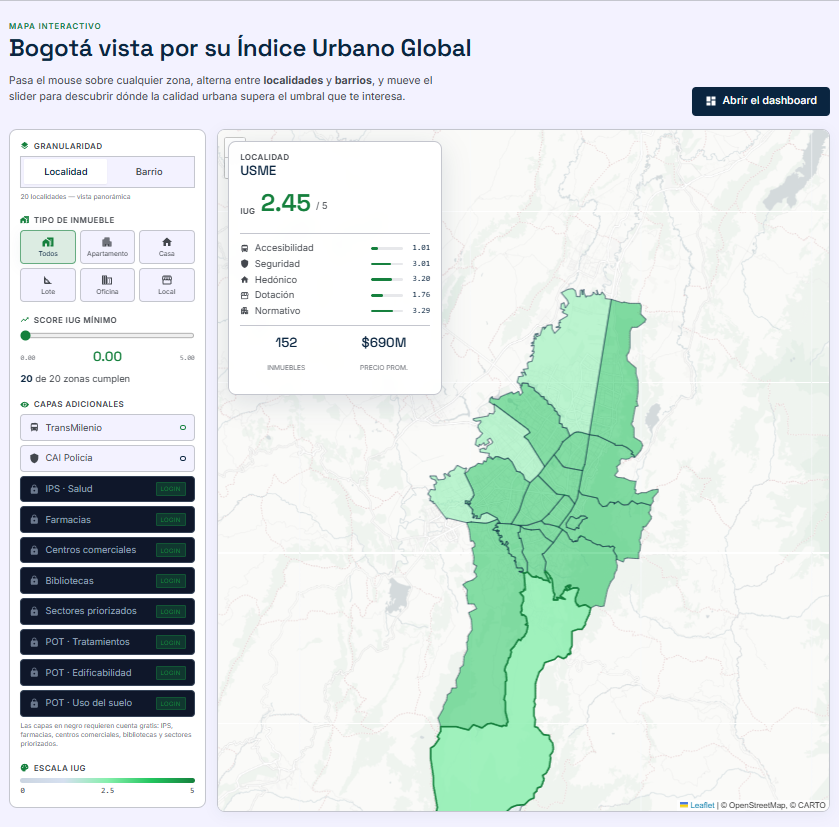
\includegraphics[width=0.85\textwidth]{figs/dashboard.png}
\caption{Interfaz de la plataforma INMU. La vista combina el mapa coroplético con un panel de filtros y el asistente conversacional, materializando el objetivo de democratización del acceso planteado en la Sección~\ref{ch:intro}.}
\label{fig:dashboard_inmu}
\end{figure}

Este módulo cumple el objetivo de democratización del acceso planteado en la Sección~\ref{ch:intro}: un usuario sin conocimiento técnico puede explorar el $\IUG$, identificar oportunidades y comparar entornos urbanos sin necesidad de consultar bases de datos directamente ni interpretar tablas estadísticas.

\section{Generación de cotizaciones (ACM)}\label{sec:cotizaciones}

Como cierre operativo del sistema, la plataforma incluye un módulo de generación automatizada de Análisis Comparativos de Mercado (ACM) en formato PDF. Dado un inmueble objetivo, el sistema selecciona comparables mediante similitud espacial y estructural, calcula intervalos de confianza con distribución $t$-Student de acuerdo con el protocolo descrito en la Sección~\ref{subsec:lectura_rlm}, y genera un documento profesional que sintetiza el desglose de los cinco subíndices del $\IUG$, el residual hedónico, el cuadrante de decisión asignado y la valoración estimada con su banda de confianza al 90\,\%.

Este módulo materializa la transición \emph{indicador} $\to$ \emph{documento operativo}: el resultado del análisis no se queda en una pantalla sino que se entrega en un formato auditable, archivable y alineado con las prácticas del sector inmobiliario profesional. Se cierra así el bucle conceptual que organiza el sistema: \emph{datos} $\to$ \emph{indicador} $\to$ \emph{decisión} $\to$ \emph{documento operativo}.

\begin{figure}[htbp]
\centering
\includegraphics[width=0.65\textwidth]{cotizacion_sample.png}
\caption{Cotización ACM generada por el sistema. Incluye comparables seleccionados, desglose del $\IUG$ por subíndices, residual hedónico, intervalo de confianza al 90\,\% (distribución $t$-Student) y cuadrante de decisión.}
\label{fig:cotizacion_sample}
\end{figure}

El PDF generado es portable, no requiere conexión persistente al sistema, y puede ser entregado como anexo a un avalúo profesional, soporte para una decisión de inversión o documentación interna de un fondo inmobiliario. Un sample real generado a partir de un inmueble del dataset se encuentra disponible en el repositorio del proyecto bajo \texttt{samples/cotizacion\_ejemplo.pdf}.



\begin{thebibliography}{99}
\addcontentsline{toc}{chapter}{Referencias consultadas}

\noindent\textit{El presente listado integra tanto las obras citadas directamente en el cuerpo del documento como la literatura consultada que sustentó el desarrollo metodológico, teórico y operativo del trabajo.}
\vspace{1em}

% -- Referencias Clásicas y Teóricas --

\bibitem[Rosen(1974)]{rosen1974}
Rosen, S. (1974).
Hedonic prices and implicit markets: product differentiation in pure competition.
\textit{Journal of Political Economy, 82}(1), 34--55.
\href{https://doi.org/10.1086/260169}{https://doi.org/10.1086/260169}

\bibitem[Hansen(1959)]{hansen1959}
Hansen, W. G. (1959).
How Accessibility Shapes Land Use.
\textit{Journal of the American Institute of Planners, 25}(2), 73--76.
\href{https://doi.org/10.1080/01944365908978307}{https://doi.org/10.1080/01944365908978307}

\bibitem[Anselin(1995)]{anselin1995}
Anselin, L. (1995).
Local Indicators of Spatial Association—LISA.
\textit{Geographical Analysis, 27}(2), 93--115.
\href{https://doi.org/10.1111/j.1538-4632.1995.tb00900.x}{https://doi.org/10.1111/j.1538-4632.1995.tb00900.x}

\bibitem[Koenker(2005)]{koenker2005}
Koenker, R. (2005).
\textit{Quantile Regression}.
Cambridge University Press.
\href{https://doi.org/10.1017/CBO9780511754098}{https://doi.org/10.1017/CBO9780511754098}

% -- Referencias de Validación y Machine Learning --

\bibitem[Mostofi et~al.(2022)]{mostofi2022}
Mostofi, F., Toğan, V., \& Başağa, H. B. (2022).
Real-estate price prediction with deep neural network and principal component analysis.
\textit{Organization, Technology and Management in Construction, 14}(1), 2568--2580.
\href{https://doi.org/10.2478/otmcj-2022-0016}{https://doi.org/10.2478/otmcj-2022-0016}

\bibitem[Cajias(2019)]{cajias2019}
Cajias, M. (2019).
Can a machine understand real estate pricing? Evaluating machine learning approaches with big data.
\textit{26th Annual European Real Estate Society Conference}. Cergy-Pontoise, France.

\bibitem[Glaeser y Gyourko(2002)]{glaeser2002}
Glaeser, E. L., \& Gyourko, J. (2002).
\textit{The Impact of Zoning on Housing Affordability} (Working Paper No. 8835).
National Bureau of Economic Research.
\href{https://doi.org/10.3386/w8835}{https://doi.org/10.3386/w8835}

\bibitem[Wheeler(2007)]{wheeler2007}
Wheeler, D. C. (2007).
Diagnostic tools and remedial methods for collinearity in geographically weighted regression.
\textit{Environment and Planning A, 39}(10), 2464--2481.
\href{https://doi.org/10.1068/a38325}{https://doi.org/10.1068/a38325}

\bibitem[Laney(2001)]{laney2001}
Laney, D. (2001).
3D data management: Controlling data volume, velocity and variety.
\textit{META Group Research Note, 6}(70), 1.

% -- Referencias Originales --

\bibitem[Khoshnoud et~al.(2023)]{Khoshnoud2023}
Khoshnoud, M., Sirmans, G. S., \& Zietz, E. N. (2023).
The evolution of hedonic pricing models.
\textit{Journal of Real Estate Literature, 31}(1), 1--47.
\href{https://doi.org/10.1080/09277544.2023.2201020}{https://doi.org/10.1080/09277544.2023.2201020}

\bibitem[Cárdenas(2017)]{Cardenas2017}
Cárdenas O’Byrne, S. (2017).
Medir el uso del espacio público urbano seguro.
\textit{Sociedad y Economía}, (33), 11--250.

\bibitem[IGAC(2024)]{IGAC1912}
Instituto Geográfico Agustín Codazzi. (2024, 6 de diciembre).
\textit{Resolución 1912 de 2024: Por medio del cual se adopta la metodología para la actualización masiva de valores catastrales rezagados}.
Recuperado de: \url{https://www.igac.gov.co/transparencia-y-acceso-a-la-informacion-publica/normograma/resolucion-1912-de-2024}

\bibitem[Haynes y Fotheringham(1985)]{HaynesFotheringham1985}
Haynes, K.~E., \& Fotheringham, A.~S. (1985).
\textit{Gravity and Spatial Interaction Models}.
Beverly Hills, CA: Sage Publications.

\bibitem[Tasadorfiable(2025)]{TasadorResidual}
Tasadorfiable. (2025, 27 de mayo).
\textit{Método de valoración residual dinámico: qué es y cómo se calcula}.
Recuperado de: \url{https://tasadorfiable.es/metodo-de-valoracion-residual-dinamico/}

% -- Referencias del Complemento Metodológico --

\bibitem[Hair et~al.(2010)]{hair2010}
Hair, J.~F., Black, W.~C., Babin, B.~J. \& Anderson, R.~E. (2010).
\textit{Multivariate Data Analysis} (7th ed.).
Pearson Prentice Hall.

\bibitem[Kaiser(1974)]{kaiser1974}
Kaiser, H.~F. (1974).
An index of factorial simplicity.
\textit{Psychometrika, 39}(1), 31--36.
\href{https://doi.org/10.1007/BF02291575}{https://doi.org/10.1007/BF02291575}

\bibitem[Bartlett(1954)]{bartlett1954}
Bartlett, M.~S. (1954).
A note on the multiplying factors for various $\chi^2$ approximations.
\textit{Journal of the Royal Statistical Society, Series B, 16}(2), 296--298.

\bibitem[Roberts et~al.(2017)]{roberts2017}
Roberts, D.~R., Bahn, V., Ciuti, S., Boyce, M.~S., Elith, J.,
Guillera-Arroita, G., \ldots\ Dormann, C.~F. (2017).
Cross-validation strategies for data with temporal, spatial, hierarchical,
or phylogenetic structure.
\textit{Ecography, 40}(8), 913--929.
\href{https://doi.org/10.1111/ecog.02881}{https://doi.org/10.1111/ecog.02881}

\bibitem[Student(1908)]{student1908}
Student [Gosset, W.~S.] (1908).
The probable error of a mean.
\textit{Biometrika, 6}(1), 1--25.
\href{https://doi.org/10.2307/2331554}{https://doi.org/10.2307/2331554}

\bibitem[Cámara de Comercio de Bogotá(2024)]{ccb2024}
Cámara de Comercio de Bogotá (2024).
\textit{Encuesta de Percepción y Victimización (EPV) 2024}. $n = 19\,354$.

\bibitem[IAAO(2013)]{iaao2013}
International Association of Assessing Officers (2013).
\textit{Standard on Ratio Studies}.
Kansas City, MO: IAAO.

\bibitem[Ester et~al.(1996)]{ester1996}
Ester, M., Kriegel, H.-P., Sander, J. \& Xu, X. (1996).
A density-based algorithm for discovering clusters in large spatial
databases with noise.
\textit{Proc. KDD-96}, 226--231.

\bibitem[Tobler(1970)]{tobler1970}
Tobler, W.~R. (1970).
A computer movie simulating urban growth in the Detroit region.
\textit{Economic Geography, 46}(sup1), 234--240.
\href{https://doi.org/10.2307/143141}{https://doi.org/10.2307/143141}

% -- Referencias del Capítulo de Validez de Uso --

\bibitem[Shiller(2015)]{shiller2015}
Shiller, R.~J. (2015).
\textit{Irrational Exuberance} (3a ed.).
Princeton University Press.
Marco conceptual del \emph{mispricing} en mercados de activos, incluyendo inmobiliario.

\bibitem[Nardo et~al.(2008)]{nardo2008}
Nardo, M., Saisana, M., Saltelli, A., Tarantola, S., Hoffman, A. \& Giovannini, E. (2008).
\textit{Handbook on Constructing Composite Indicators: Methodology and User Guide}.
OECD Publishing.
\href{https://doi.org/10.1787/9789264043466-en}{https://doi.org/10.1787/9789264043466-en}

\bibitem[Nimon \& Oswald(2013)]{nimon2013}
Nimon, K.~F. \& Oswald, F.~L. (2013).
Understanding the results of multiple linear regression: beyond standardized regression coefficients.
\textit{Organizational Research Methods, 16}(4), 650--674.
\href{https://doi.org/10.1177/1094428113493929}{https://doi.org/10.1177/1094428113493929}

\bibitem[Munda(2008)]{munda2008}
Munda, G. (2008).
\textit{Social Multi-Criteria Evaluation for a Sustainable Economy}.
Springer.
Discusión sobre compensatoriedad y no-compensatoriedad en agregación multicriterio.

\bibitem[Ishizaka \& Labib(2011)]{ishizaka2011}
Ishizaka, A. \& Labib, A. (2011).
Review of the main developments in the analytic hierarchy process.
\textit{Expert Systems with Applications, 38}(11), 14336--14345.
\href{https://doi.org/10.1016/j.eswa.2011.04.143}{https://doi.org/10.1016/j.eswa.2011.04.143}

\end{thebibliography}
\end{document}